\chapter{Quantification of Spatial Self-Shielding Effects}
\label{chap:quantify}


%%%%%%%%%%%%%%%%%%%%%%%%%%%%%%%%%%%%%%%%%%%%%%%%%%%%%%%%%%%%%%%%%%%%%%%%%%%%%%%
\section{Pin-wise Spatial Homogenization Schemes}
\label{sec:chap8-pinwise-space-homogenize}

\begin{figure}[h!]
\centering
\begin{subfigure}{.5\textwidth}
  \centering
  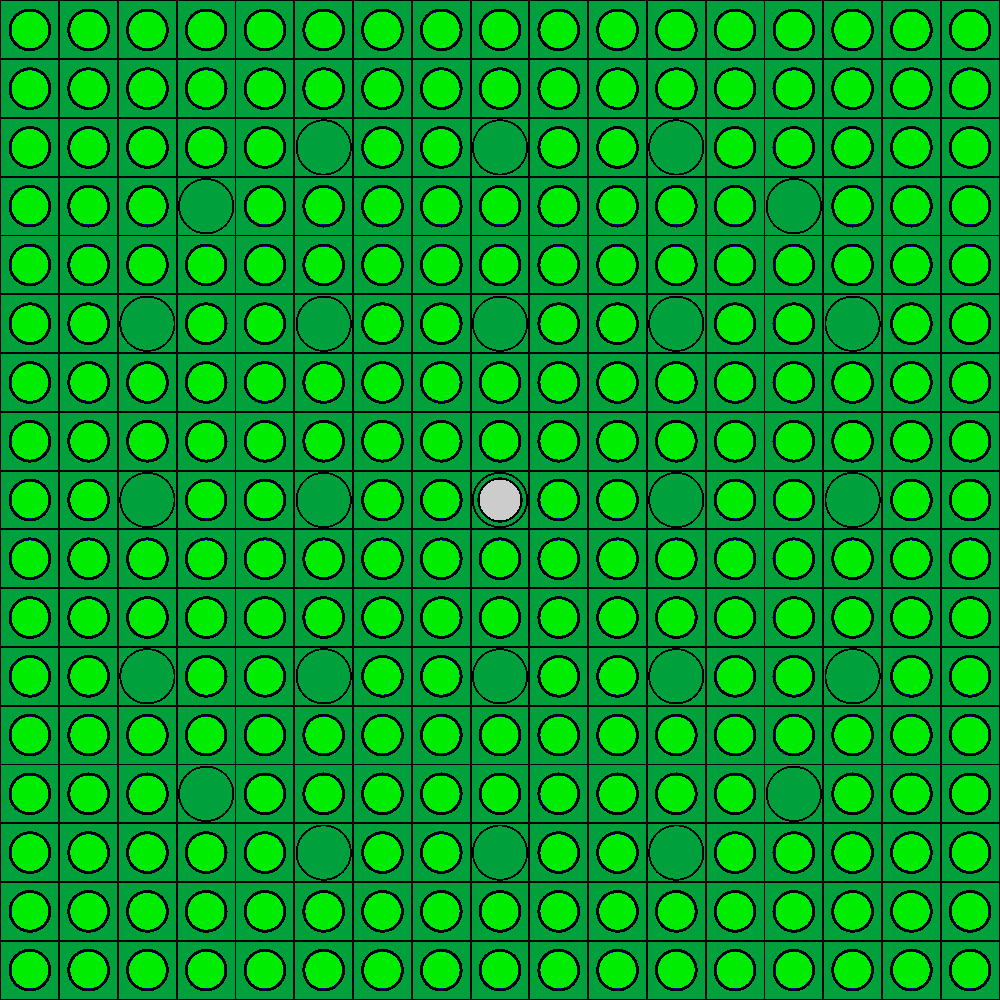
\includegraphics[width=0.9\linewidth]{figures/quantification/homogenization/assm-16-null-materials}
  \caption{}
  \label{fig:chap8-assm-16-null-materials}
\end{subfigure}%
\begin{subfigure}{.5\textwidth}
  \centering
  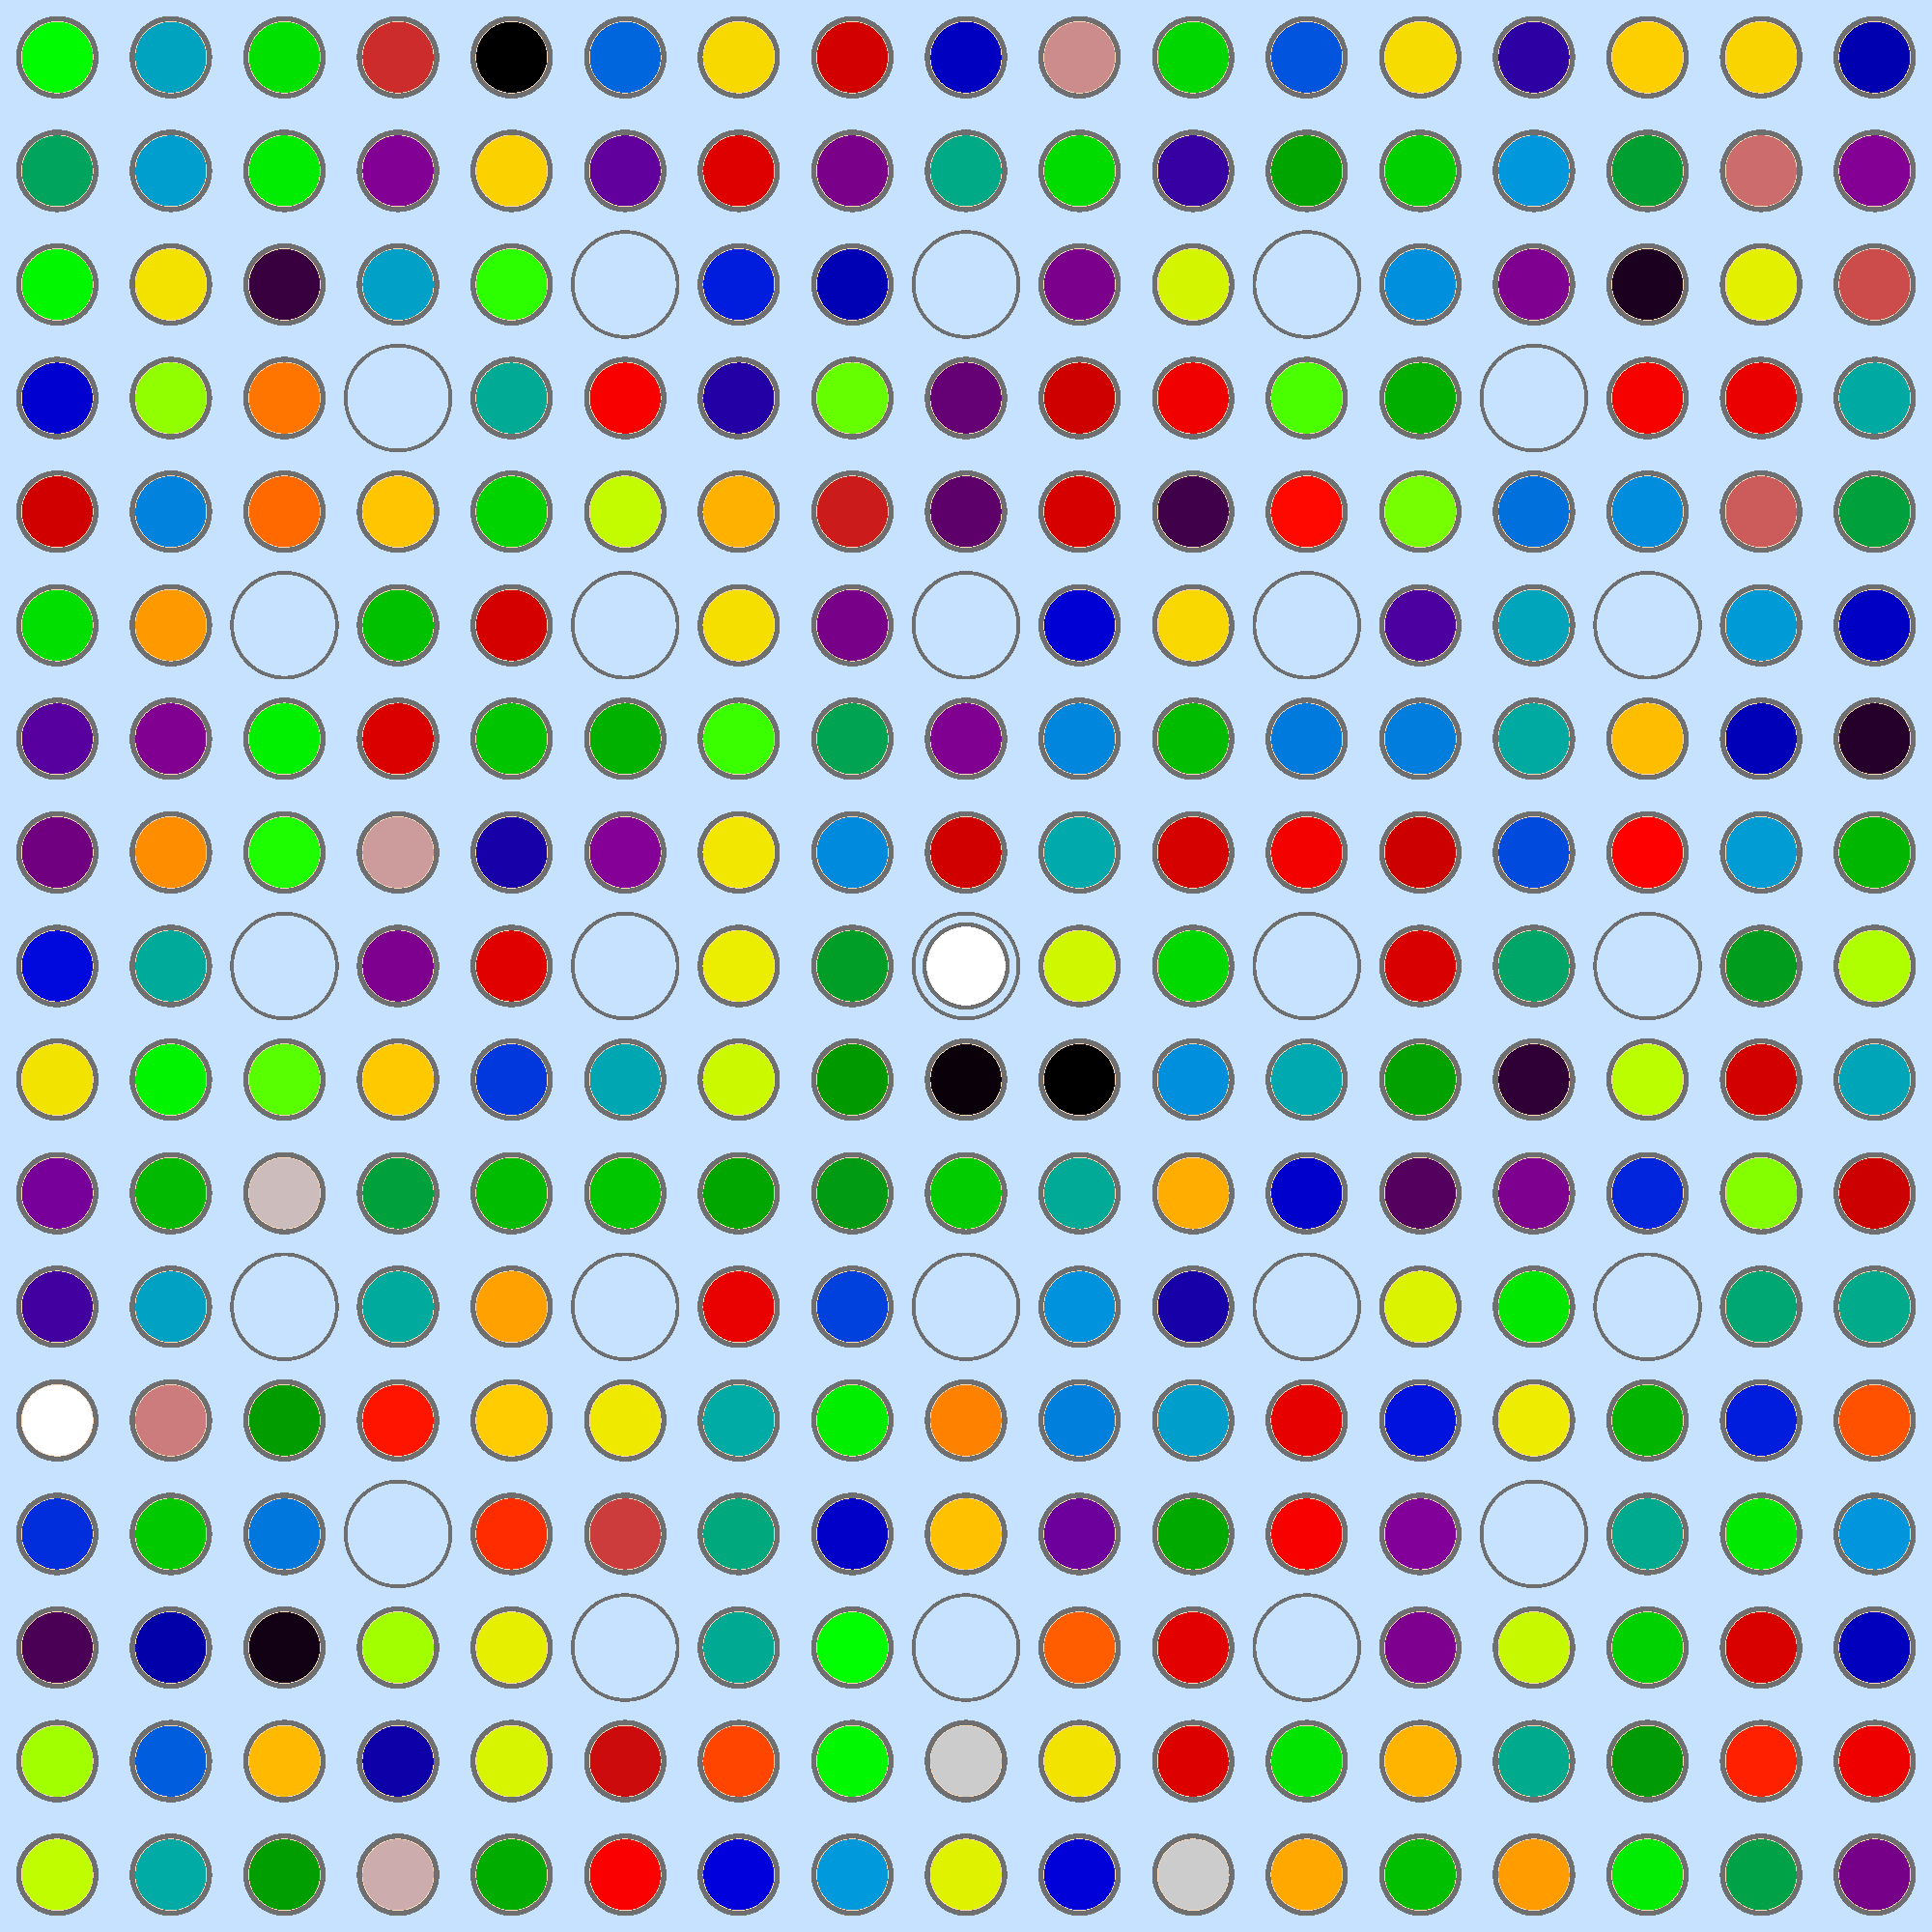
\includegraphics[width=0.9\linewidth]{figures/quantification/homogenization/assm-16-degenerate-materials}
  \caption{}
  \label{fig:chap8-assm-16-degenerate-materials}
\end{subfigure}
\begin{subfigure}{.5\textwidth}
  \centering
  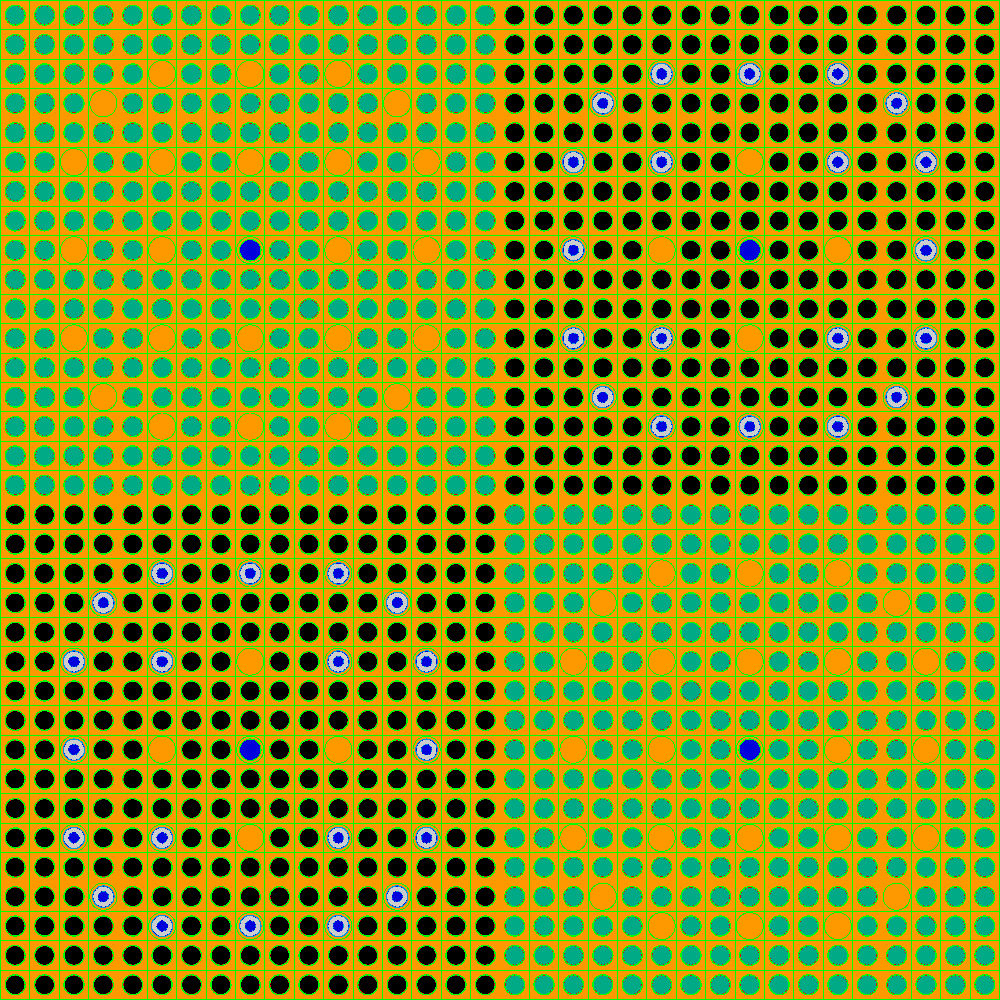
\includegraphics[width=0.9\linewidth]{figures/quantification/homogenization/2x2-null-materials}
  \caption{}
  \label{fig:chap8-2x2-null-materials}
\end{subfigure}%
\begin{subfigure}{.5\textwidth}
  \centering
  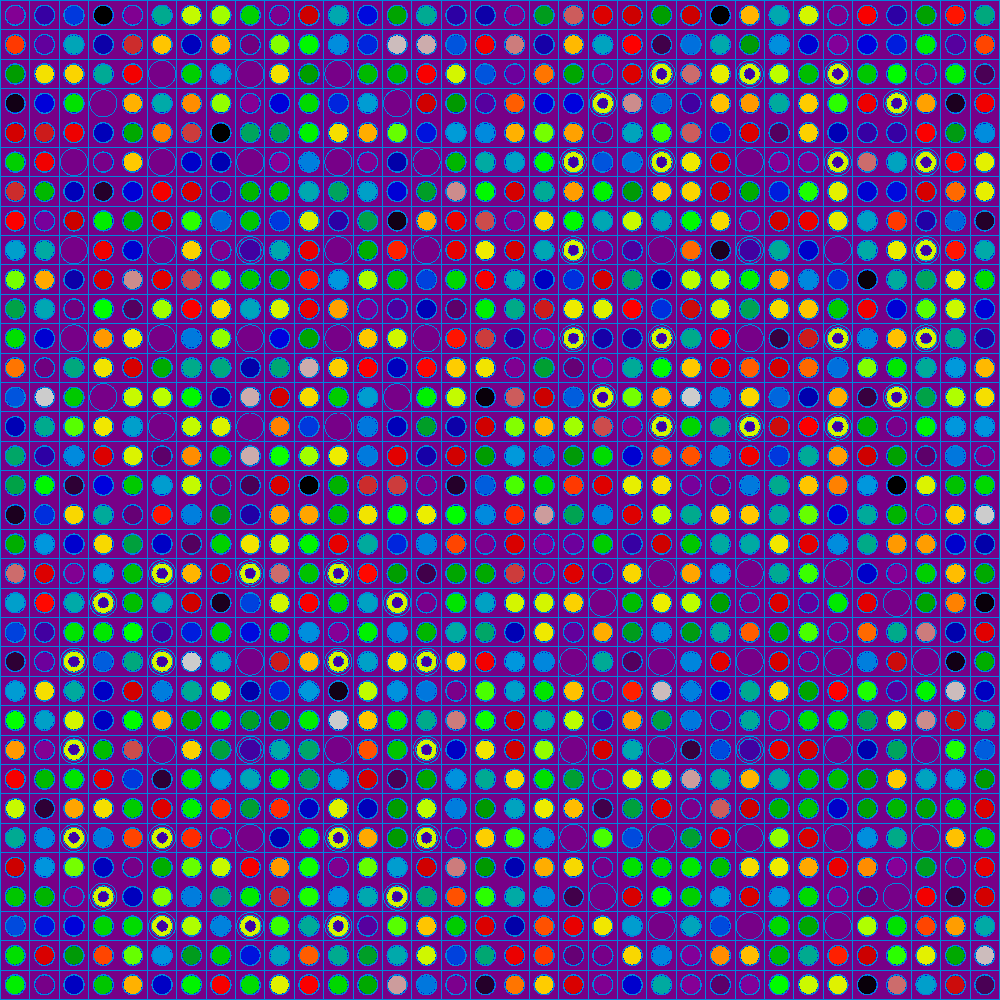
\includegraphics[width=0.9\linewidth]{figures/quantification/homogenization/2x2-degenerate-materials}
  \caption{}
  \label{fig:chap8-2x2-degenerate-materials}
\end{subfigure}
%\begin{subfigure}{.5\textwidth}
%  \centering
%  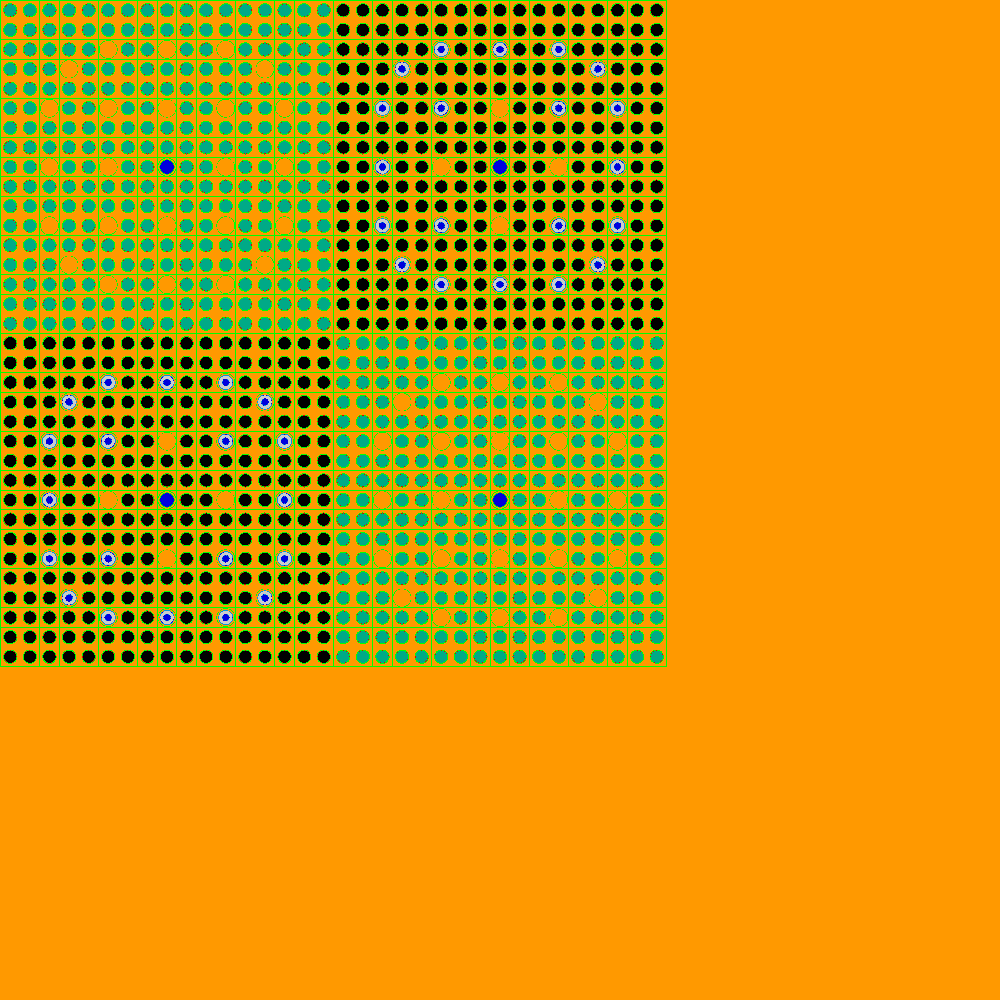
\includegraphics[width=0.9\linewidth]{figures/quantification/homogenization/reflector-null-materials}
%  \caption{}
%  \label{fig:chap8-reflector-null-materials}
%\end{subfigure}%
%\begin{subfigure}{.5\textwidth}
%  \centering
%  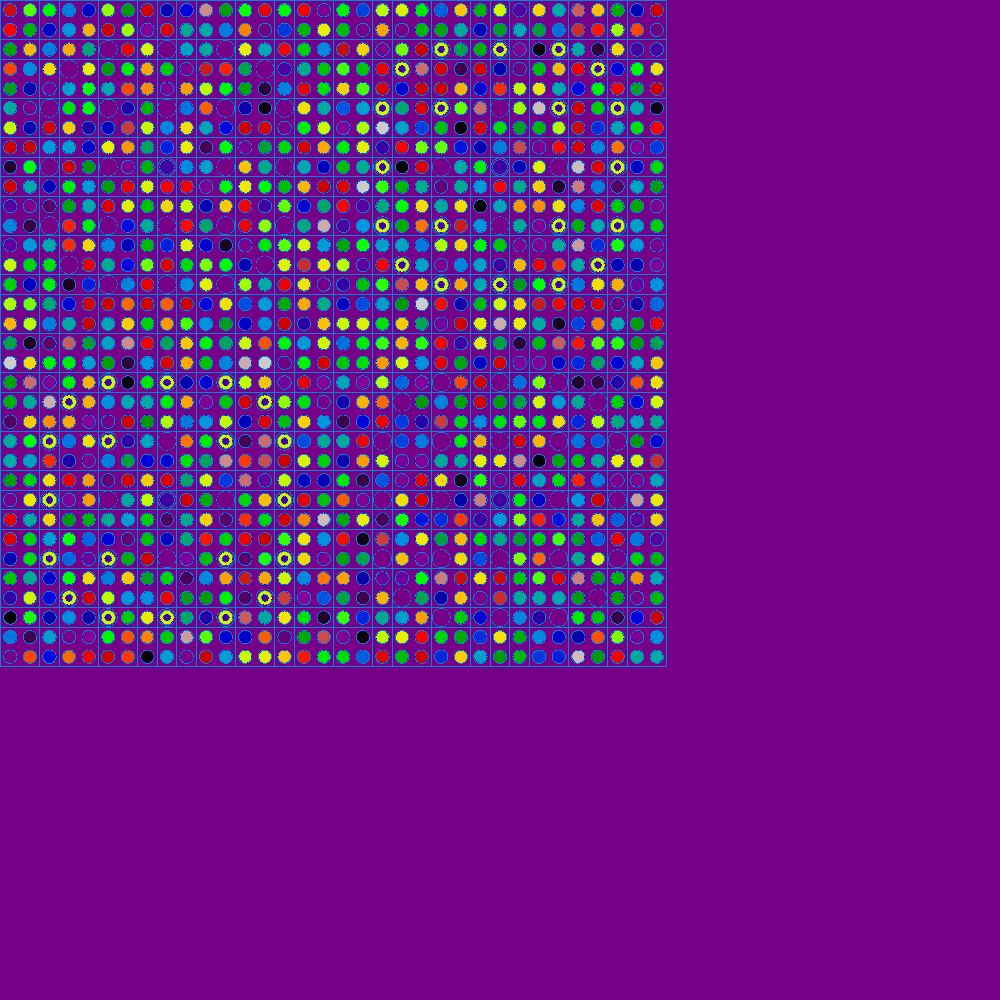
\includegraphics[width=0.9\linewidth]{figures/quantification/homogenization/reflector-degenerate-materials}
%  \caption{}
%  \label{fig:chap8-refelctor-degenerate-materials}
%\end{subfigure}
%\caption[Spatial homogenization schemes]{1.6\% enriched fuel pin (a), control rod guide tube (b), instrument tube (c) and burnable poison (d).}
\label{fig:chap8-homogenization-schemes}
\end{figure}

%%%%%%%%%%%%%%%%%%%%%%%%%%%%%%%%%%%%%%
\subsection{Infinite Lattice Homogenization}
\label{subsec:chap8-infinite}

%%%%%%%%%%%%%%%%%%%%%%%%%%%%%%%%%%%%%%
\subsection{Null Homogenization}
\label{subsec:chap8-null}

%%%%%%%%%%%%%%%%%%%%%%%%%%%%%%%%%%%%%%
\subsection{Degenerate Homogenization}
\label{subsec:chap8-degenerate}


%%%%%%%%%%%%%%%%%%%%%%%%%%%%%%%%%%%%%%%%%%%%%%%%%%%%%%%%%%%%%%%%%%%%%%%%%%%%%%%
\section{MGXS Convergence Rates}
\label{sec:chap8-mgxs-converge}

\begin{itemize}[noitemsep]
  \item Plot evolution of rel. err. by batch for each homogenization scheme
  \begin{itemize}[noitemsep]
    \item groups with highest rel. err.
    \item reactions with greatest contribution to eigenvalue (U-238 capture)
    \item total (track-length) vs. scattering matrices (analog)    
    \item which group structure(s)?
 \end{itemize}
  \item compare to pin power convergence rates in preceding chapter
\end{itemize}


%%%%%%%%%%%%%%%%%%%%%%%%%%%%%%%%%%%%%%%%%%%%%%%%%%%%%%%%%%%%%%%%%%%%%%%%%%%%%%%
\section{Flat Source Region Discretizations}
\label{sec:chap8-fsr-discretizations}

\begin{figure}[h!]
\centering
\begin{subfigure}{.5\textwidth}
  \centering
  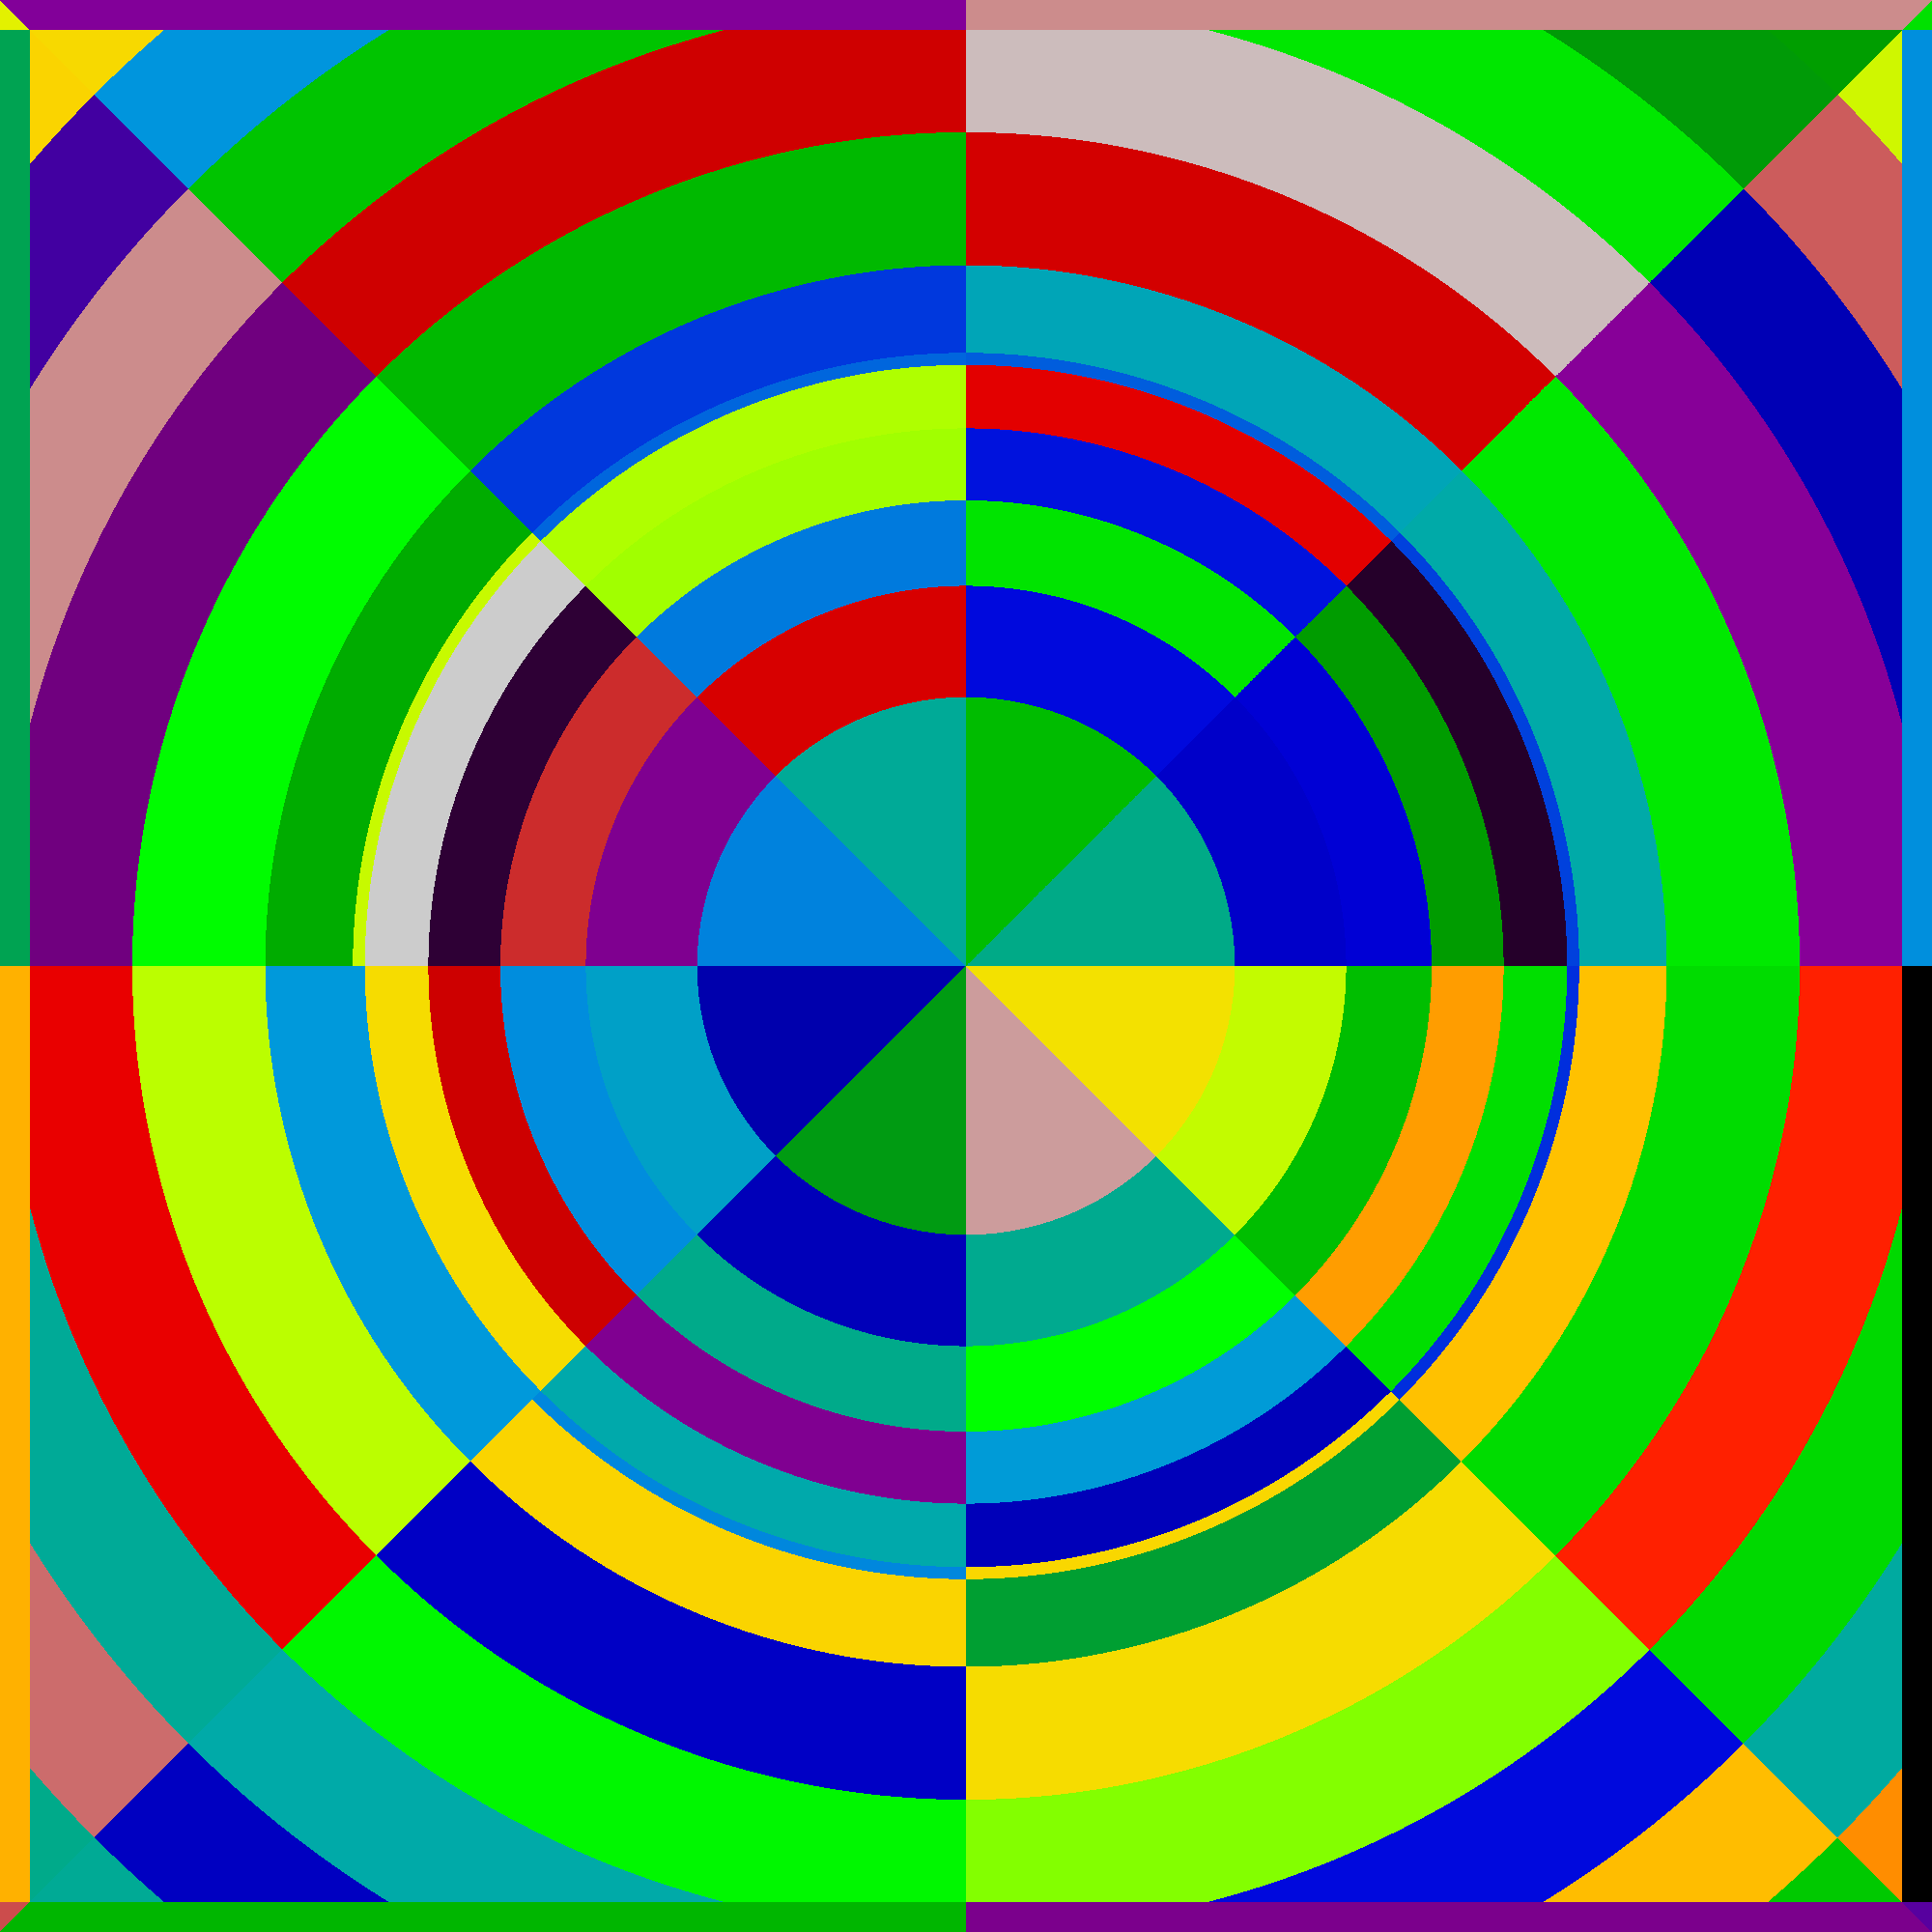
\includegraphics[width=0.9\linewidth]{figures/quantification/fsrs/fsrs-fuel-pin}
  \caption{}
  \label{fig:chap8-pin-1.6}
\end{subfigure}%
\begin{subfigure}{.5\textwidth}
  \centering
  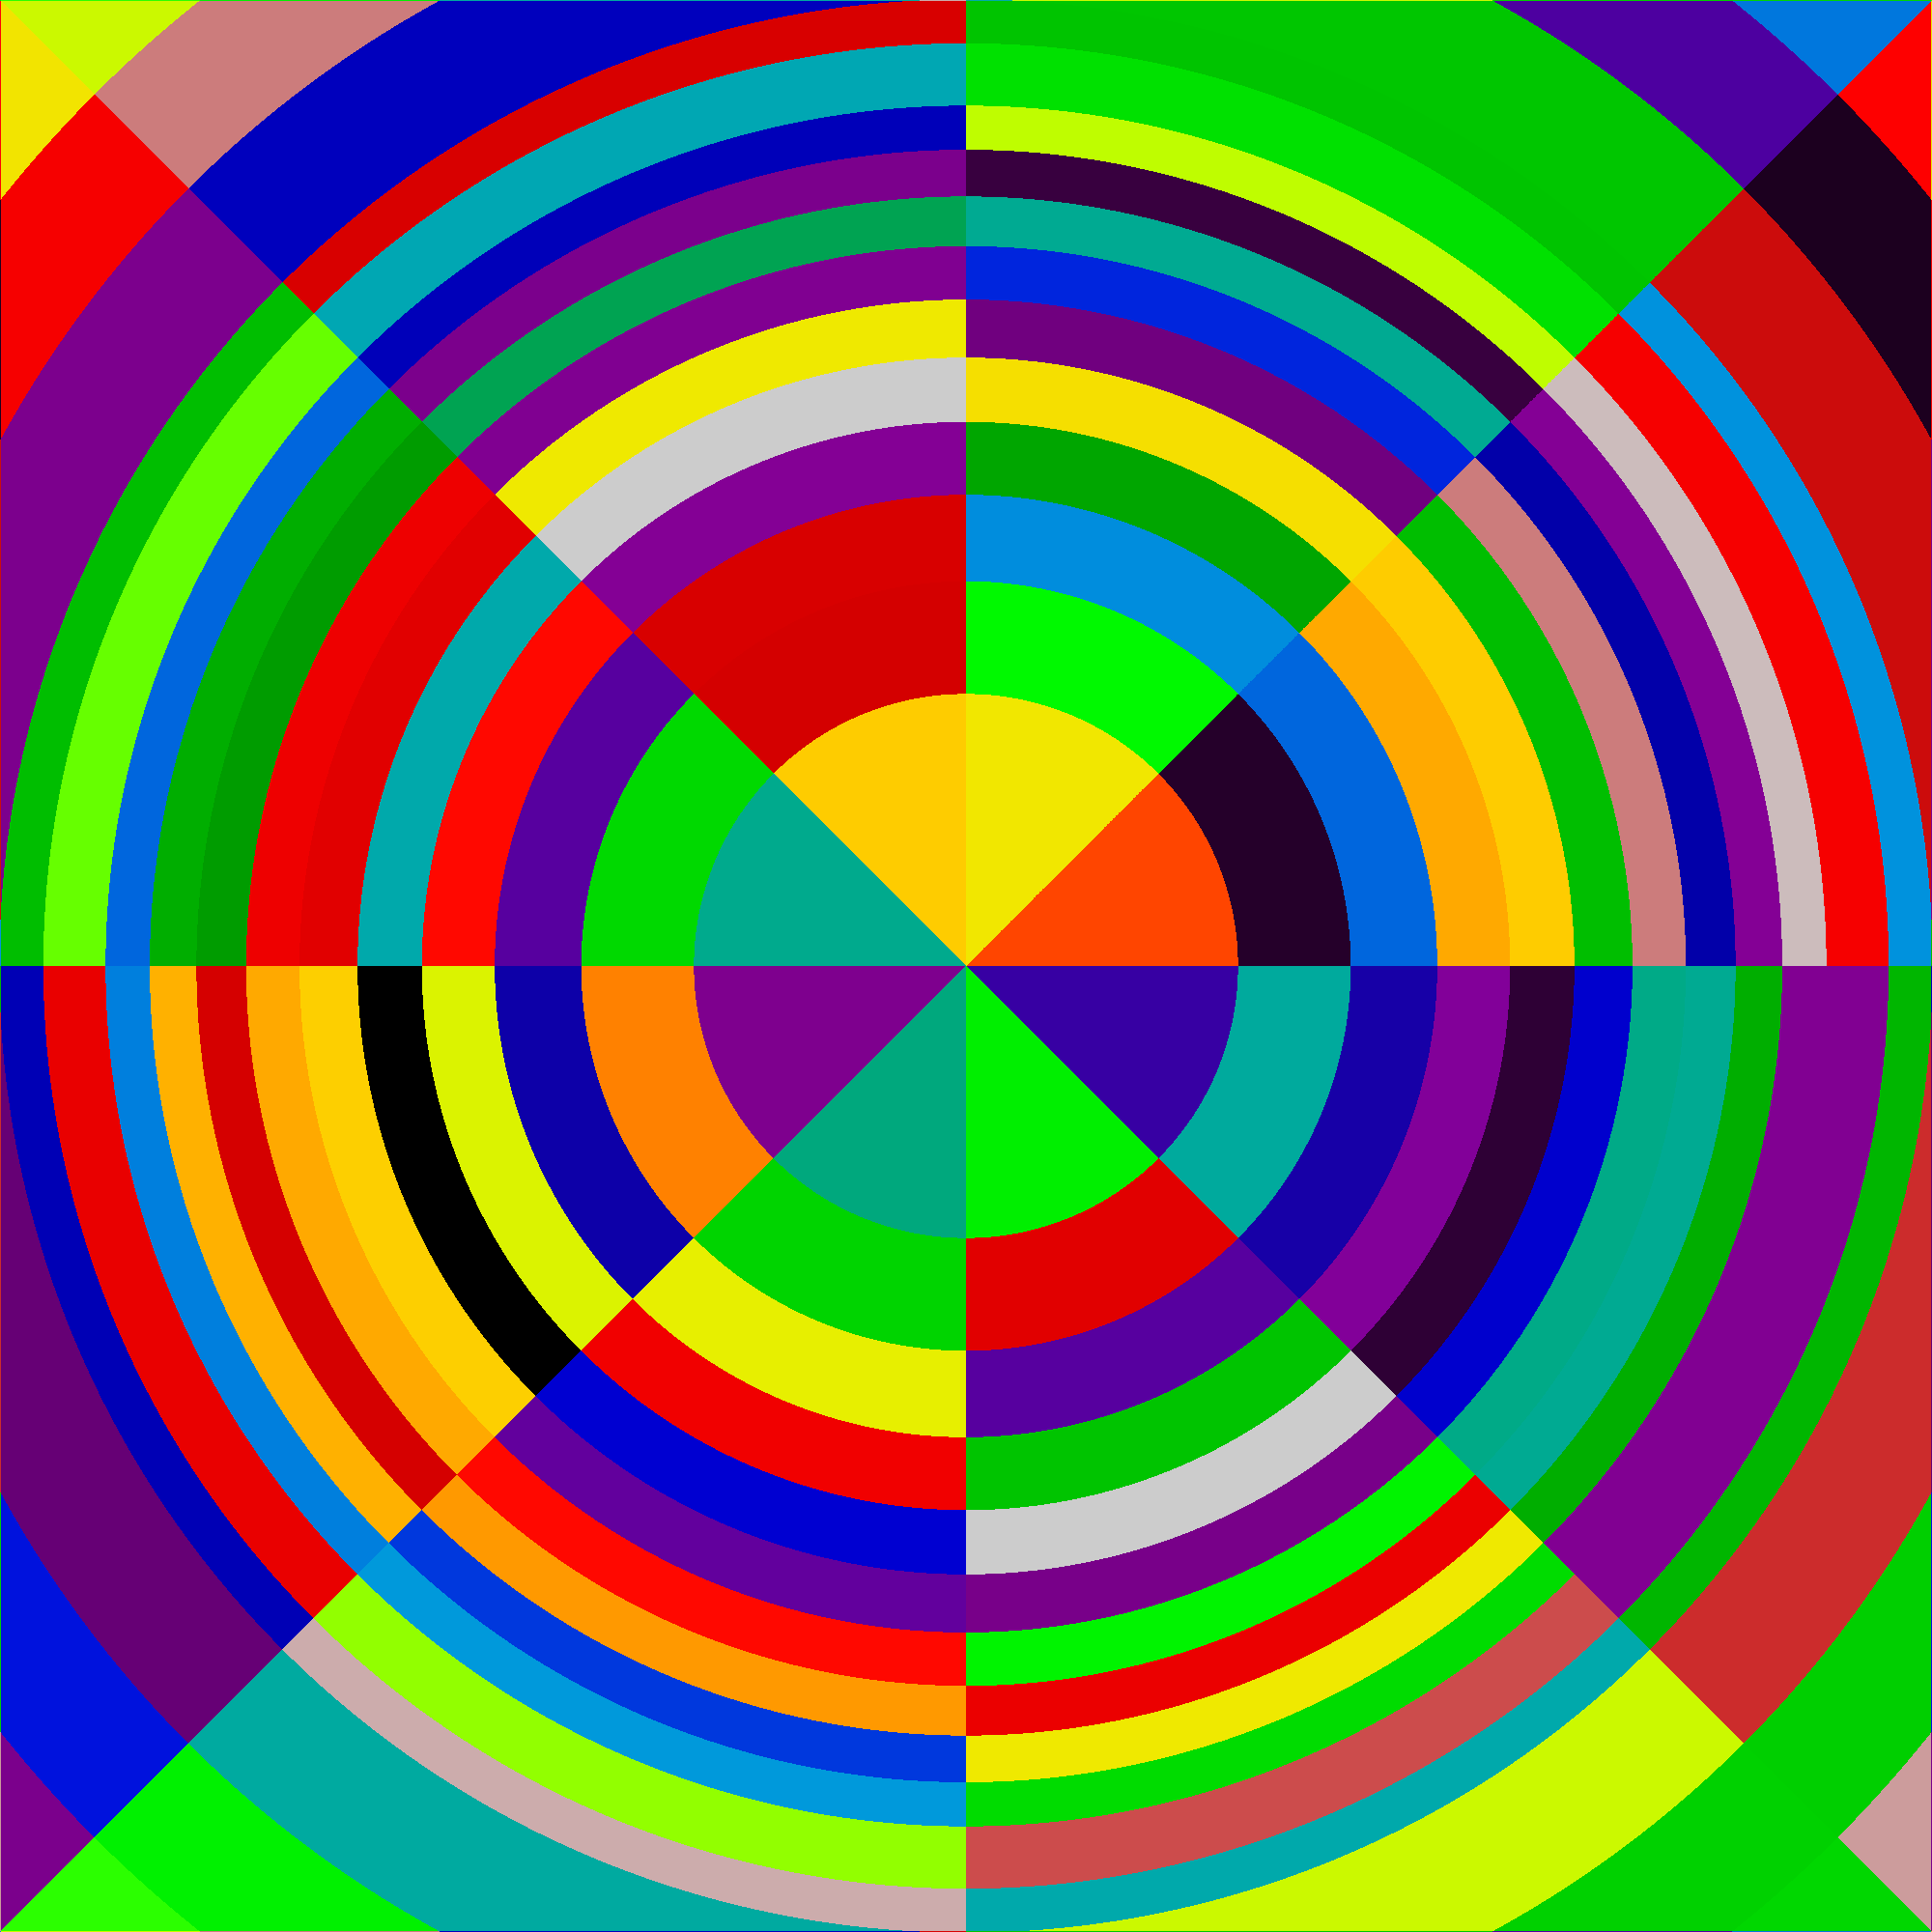
\includegraphics[width=0.9\linewidth]{figures/quantification/fsrs/fsrs-crgt}
  \caption{}
  \label{fig:chap8-pin-crgt}
\end{subfigure}
\begin{subfigure}{.5\textwidth}
  \centering
  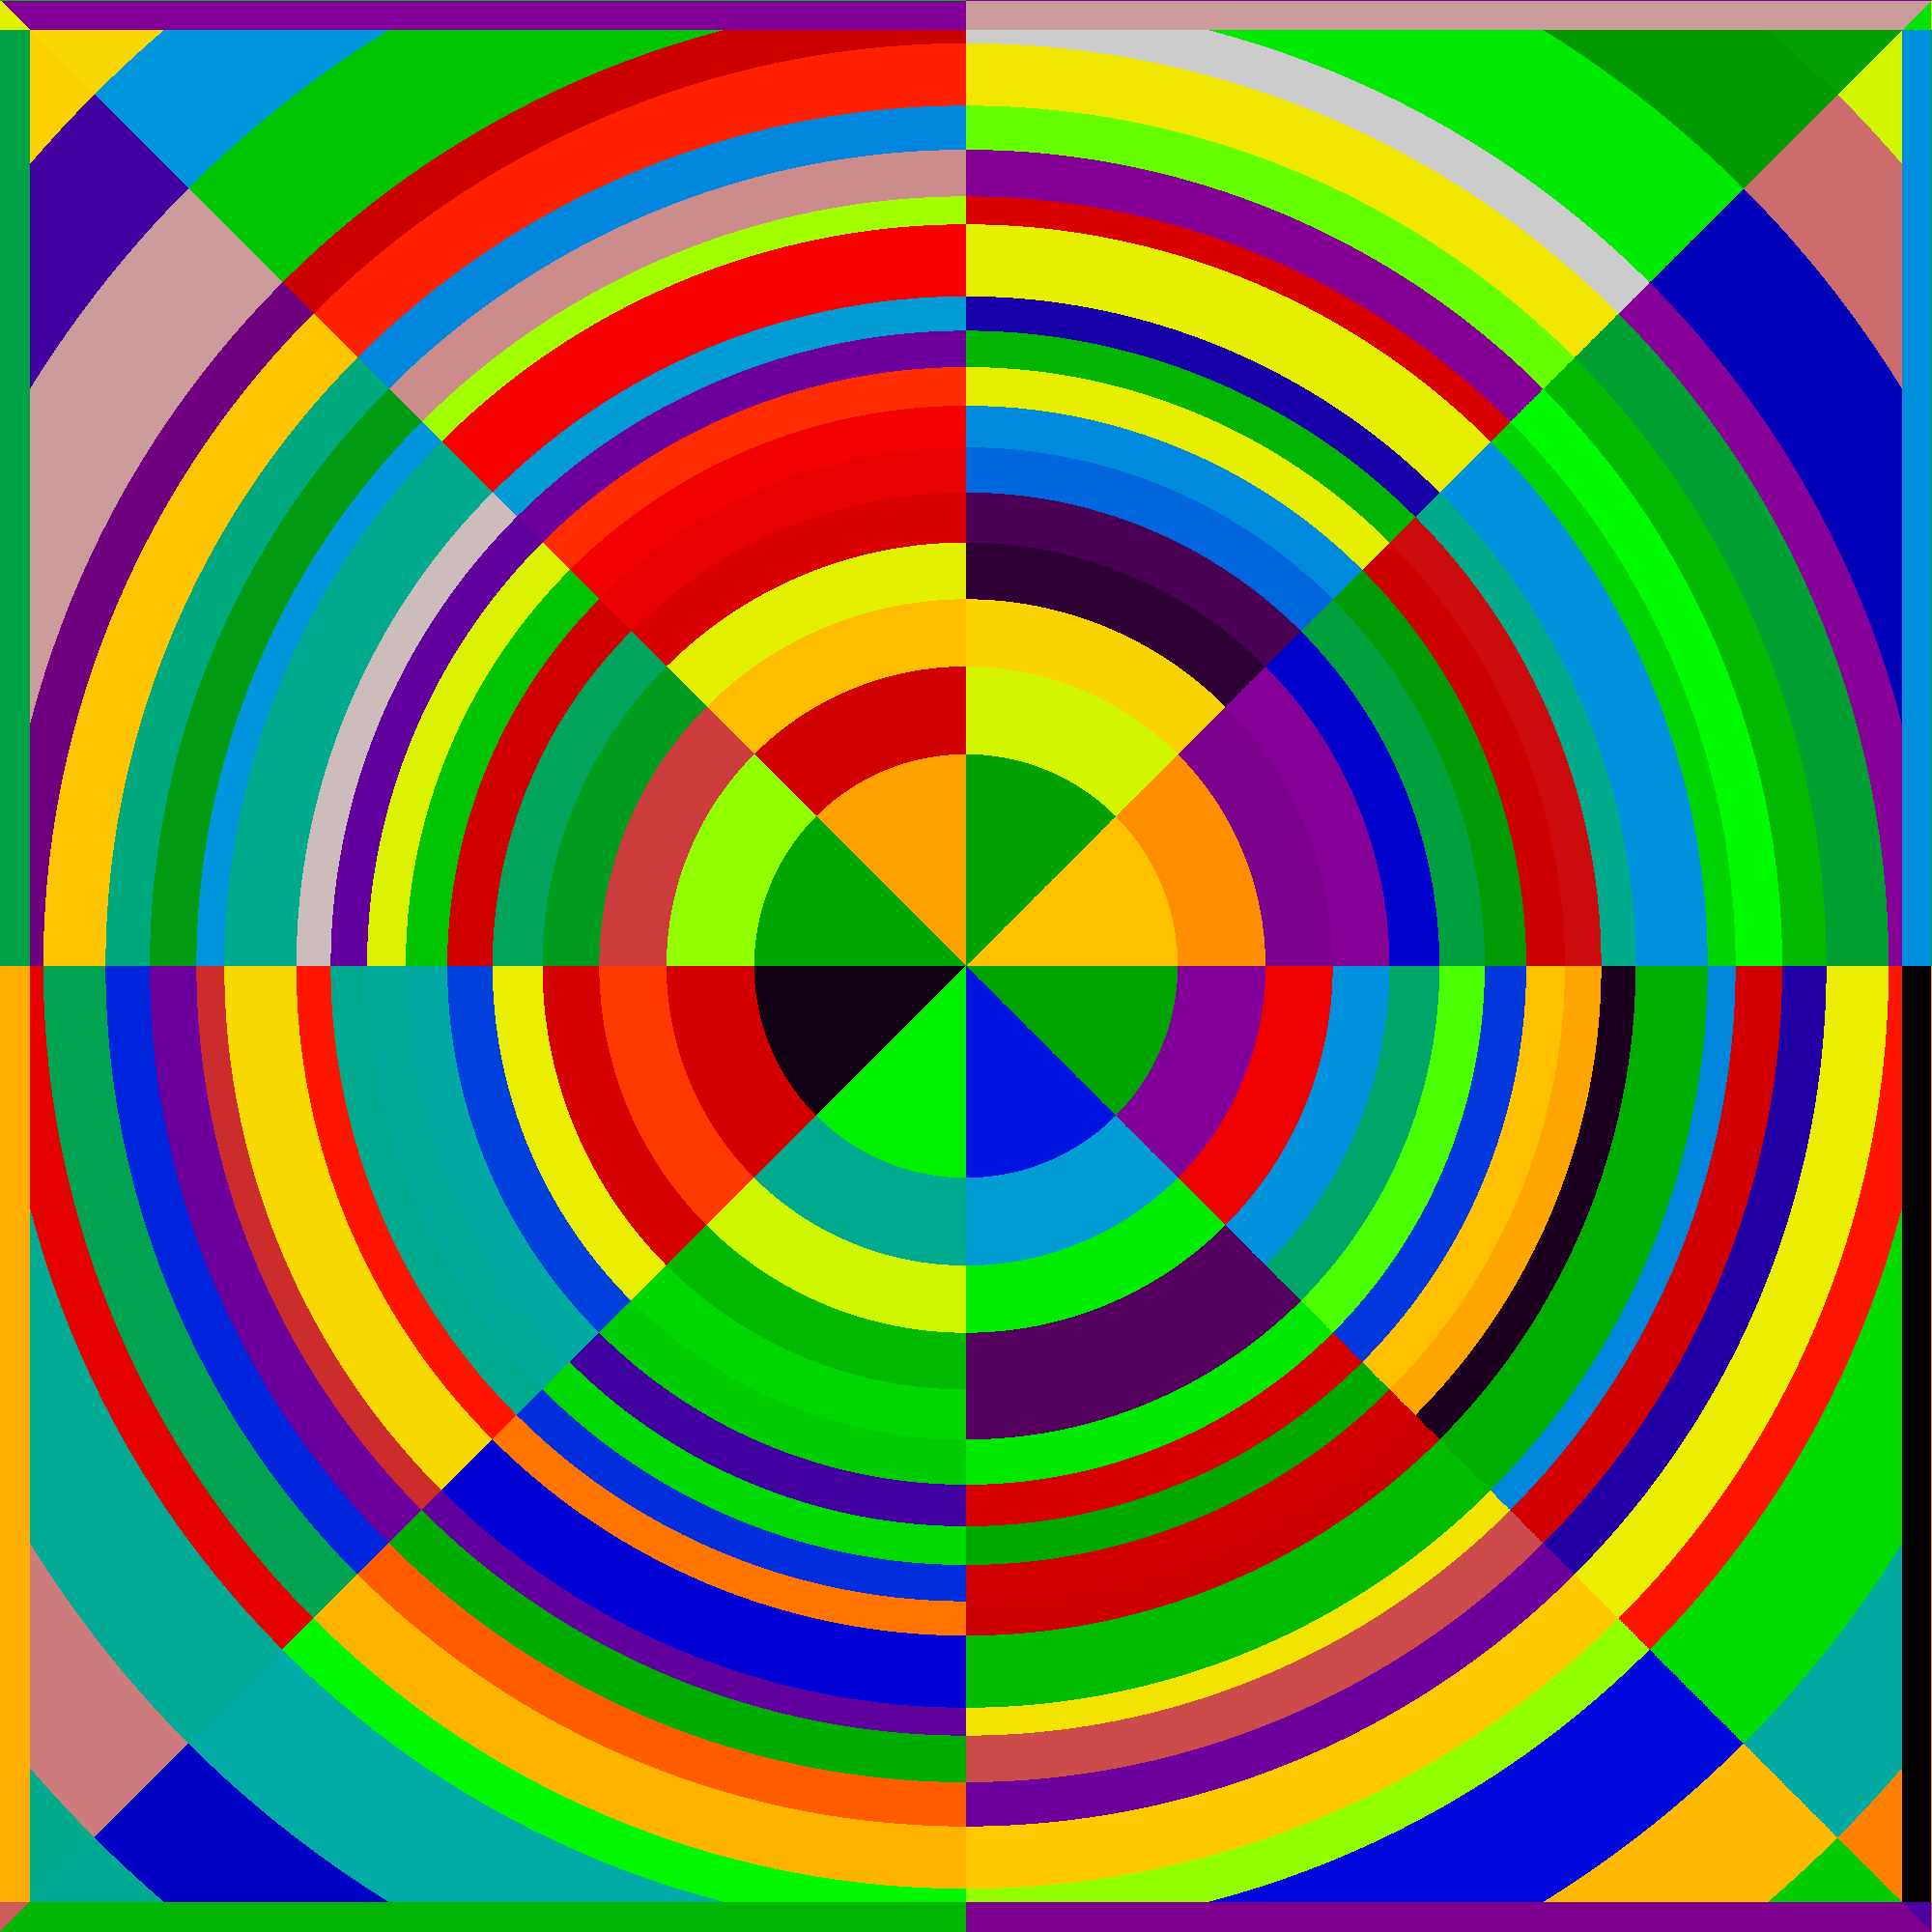
\includegraphics[width=0.9\linewidth]{figures/quantification/fsrs/fsrs-instr-tube}
  \caption{}
  \label{fig:chap8-instr-tube}
\end{subfigure}%
\begin{subfigure}{.5\textwidth}
  \centering
  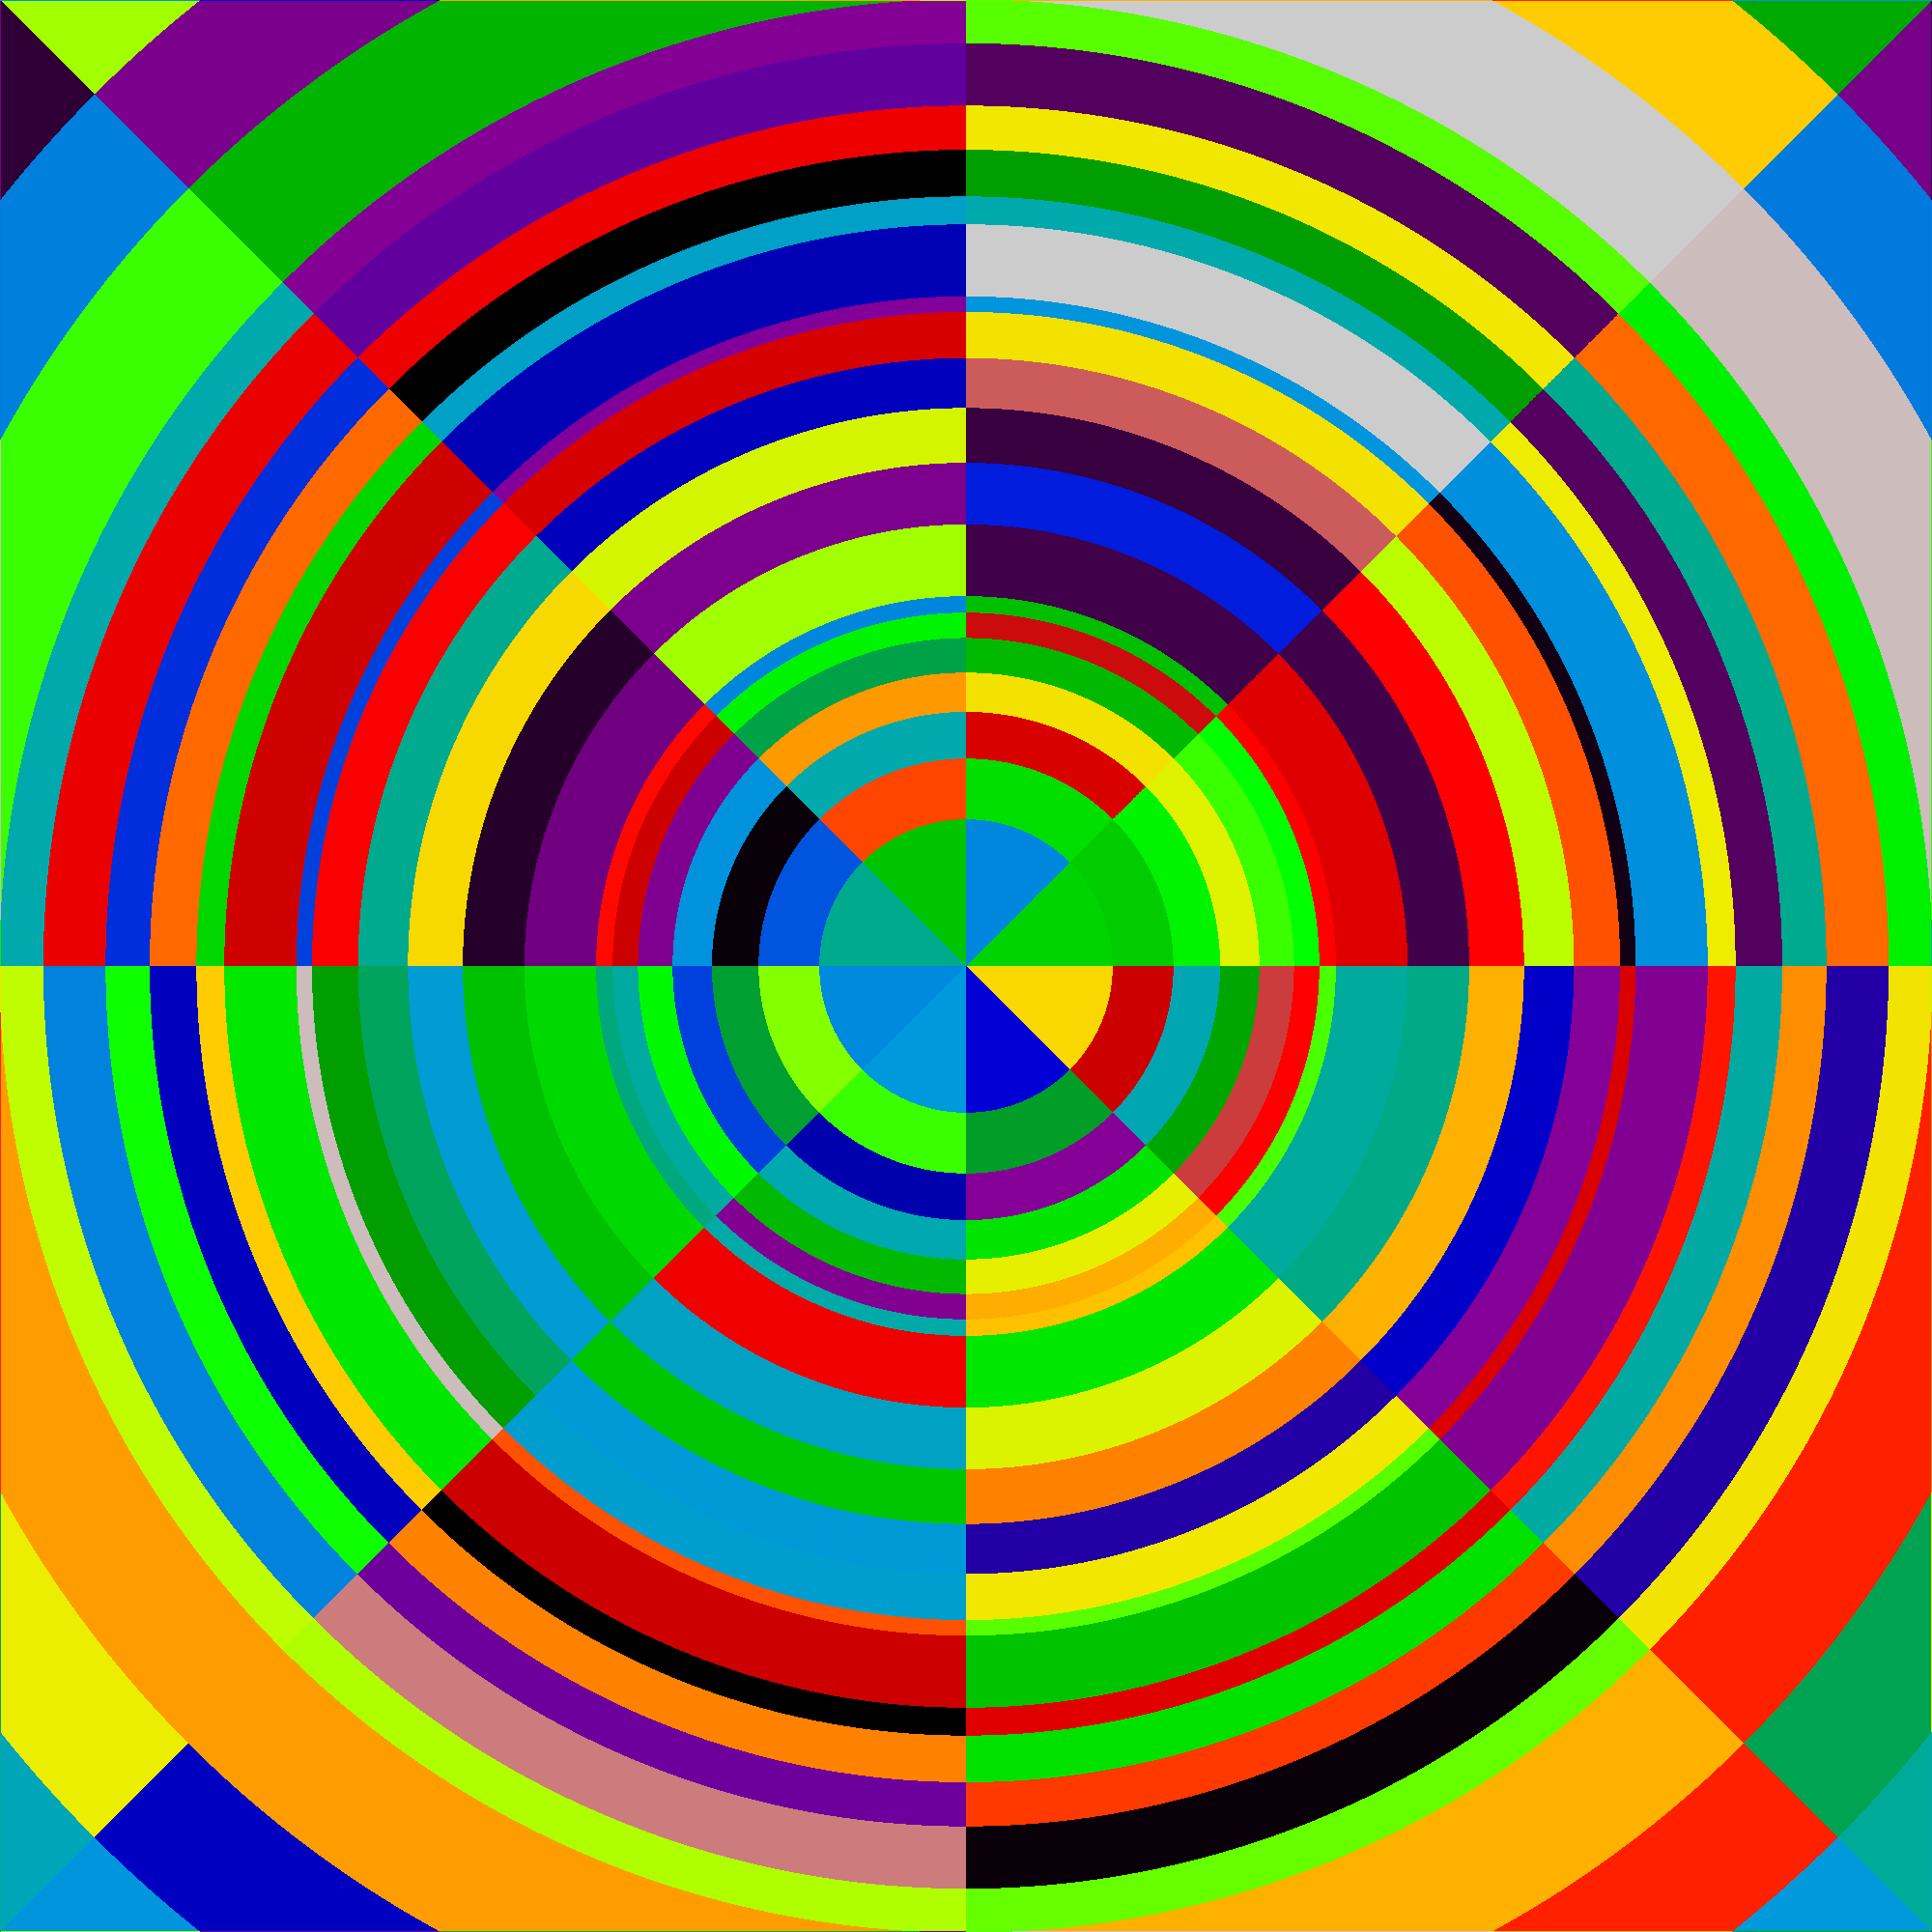
\includegraphics[width=0.9\linewidth]{figures/quantification/fsrs/fsrs-bp}
  \caption{}
  \label{fig:chap8-bp}
\end{subfigure}%
\caption[BEAVRS pin cell FSR discretization]{1.6\% enriched fuel pin (a), control rod guide tube (b), instrument tube (c) and burnable poison (d).}
\label{fig:chap8-pin-cell-fsrs}
\end{figure}

\begin{figure}[h!]
\centering
\begin{subfigure}{0.5\textwidth}
  \centering
  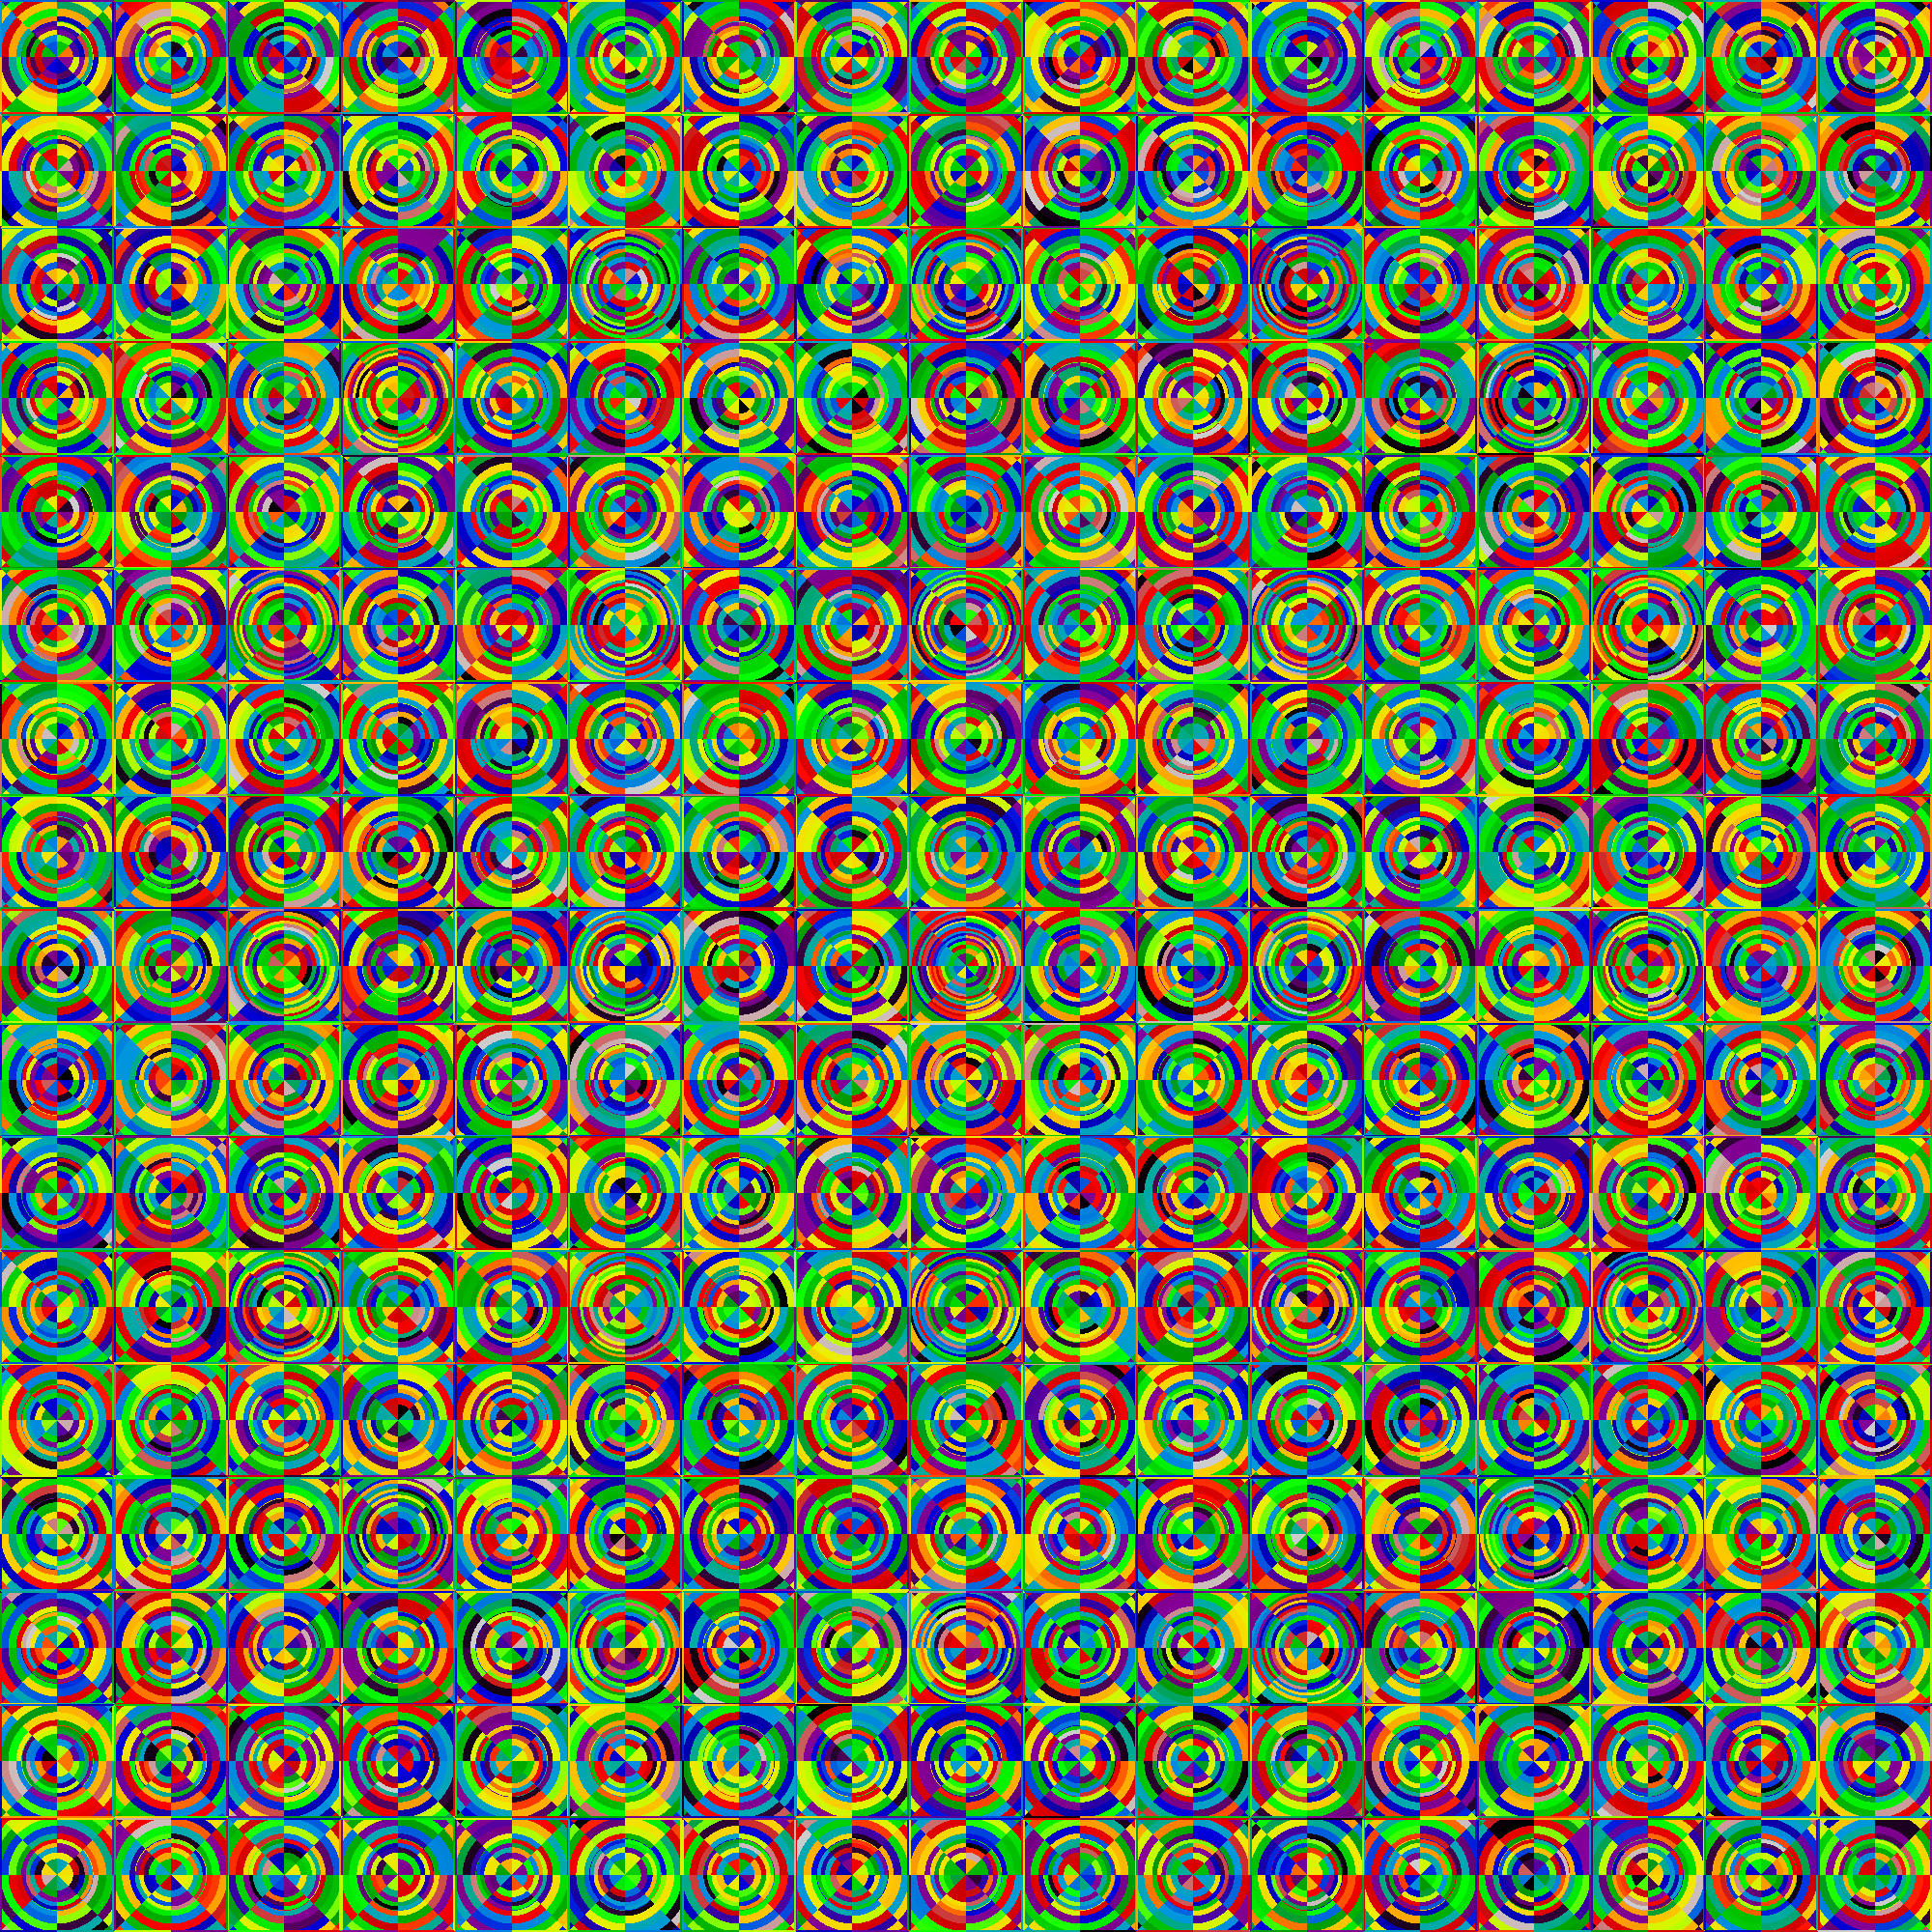
\includegraphics[width=0.9\linewidth]{figures/quantification/fsrs/fsrs-assm-16}
  \caption{}
  \label{fig:chap8-assm-1.6}
\end{subfigure}%
\begin{subfigure}{0.5\textwidth}
  \centering
  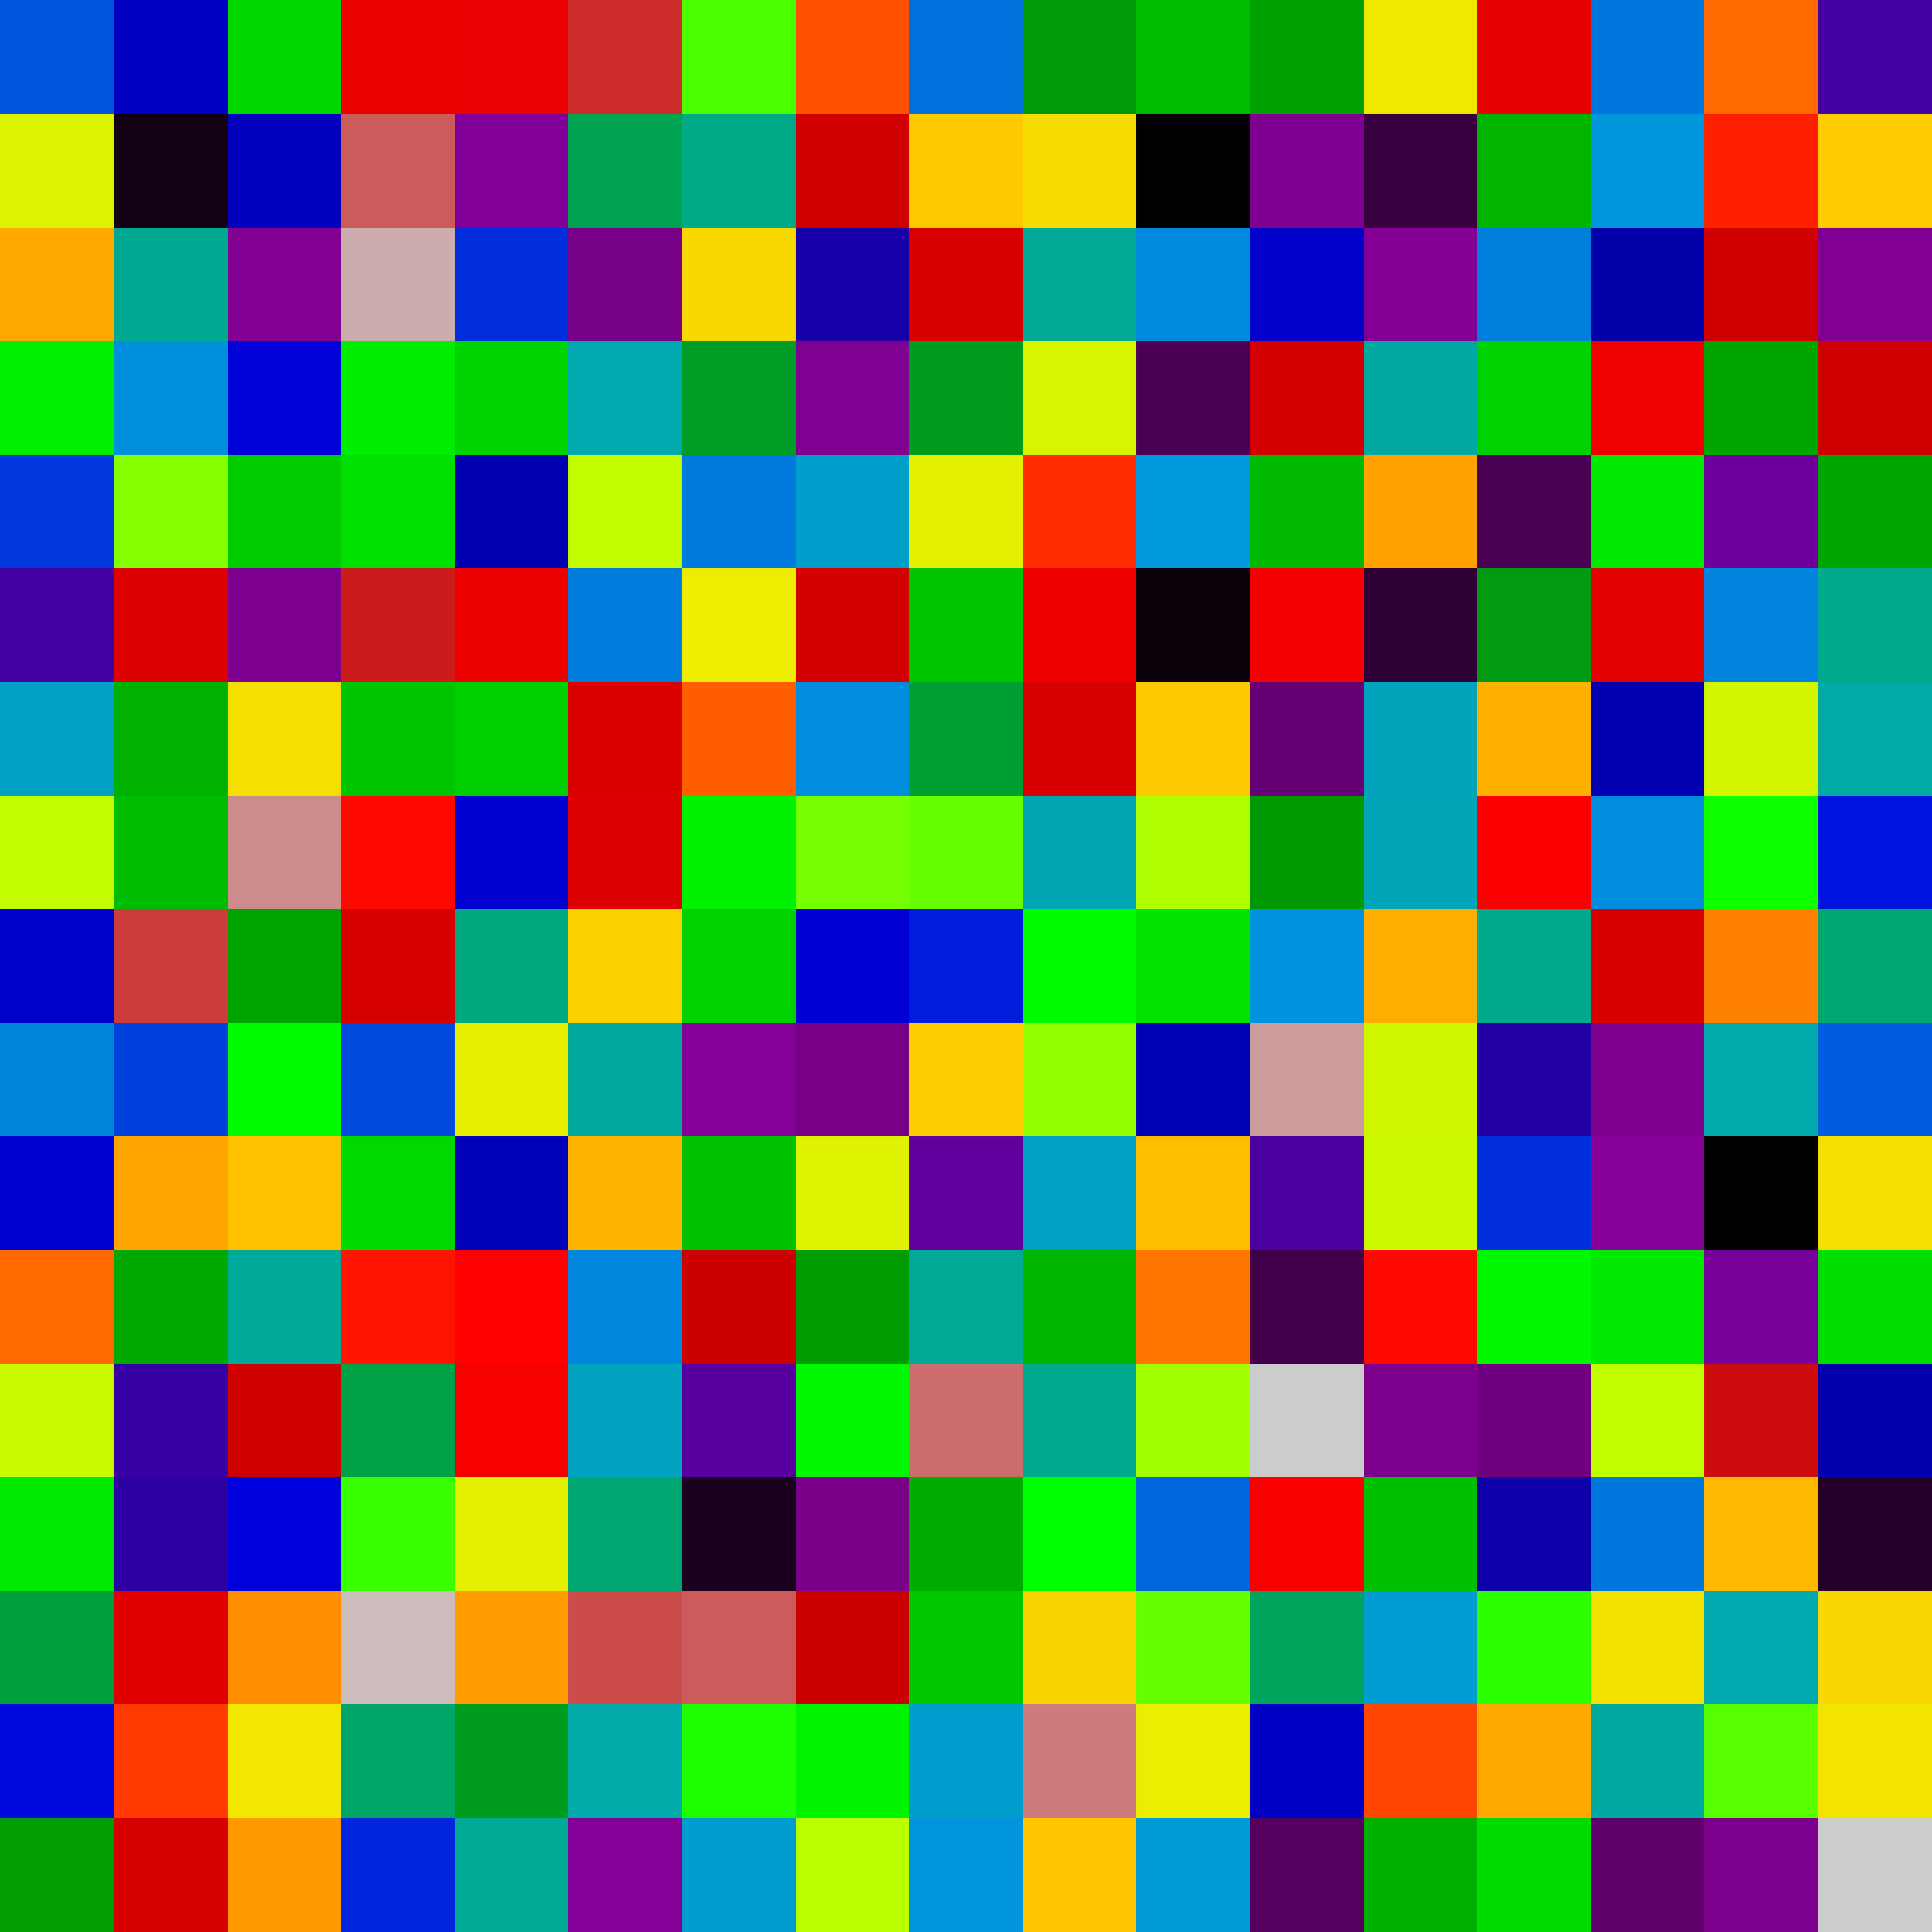
\includegraphics[width=0.9\linewidth]{figures/quantification/cmfd/cmfd-cells-assm}
  \caption{}
  \label{fig:chap8-cmfd-cells}
\end{subfigure}
\caption[FSR discretization and CMFD cells for a fuel assembly]{\ac{FSR} discretization and \ac{CMFD} cells for a fuel assembly}
\label{fig:chap8-assm-fsrs-cmfd-cells}
\end{figure}

\begin{figure}[h!]
\centering
\begin{subfigure}{0.5\textwidth}
  \centering
  
\includegraphics[width=0.9\linewidth]{figures/quantification/fsrs/fsrs-reflector}
  \caption{}
  \label{fig:chap8-assm-1.6}
\end{subfigure}%
\begin{subfigure}{0.5\textwidth}
  \centering
  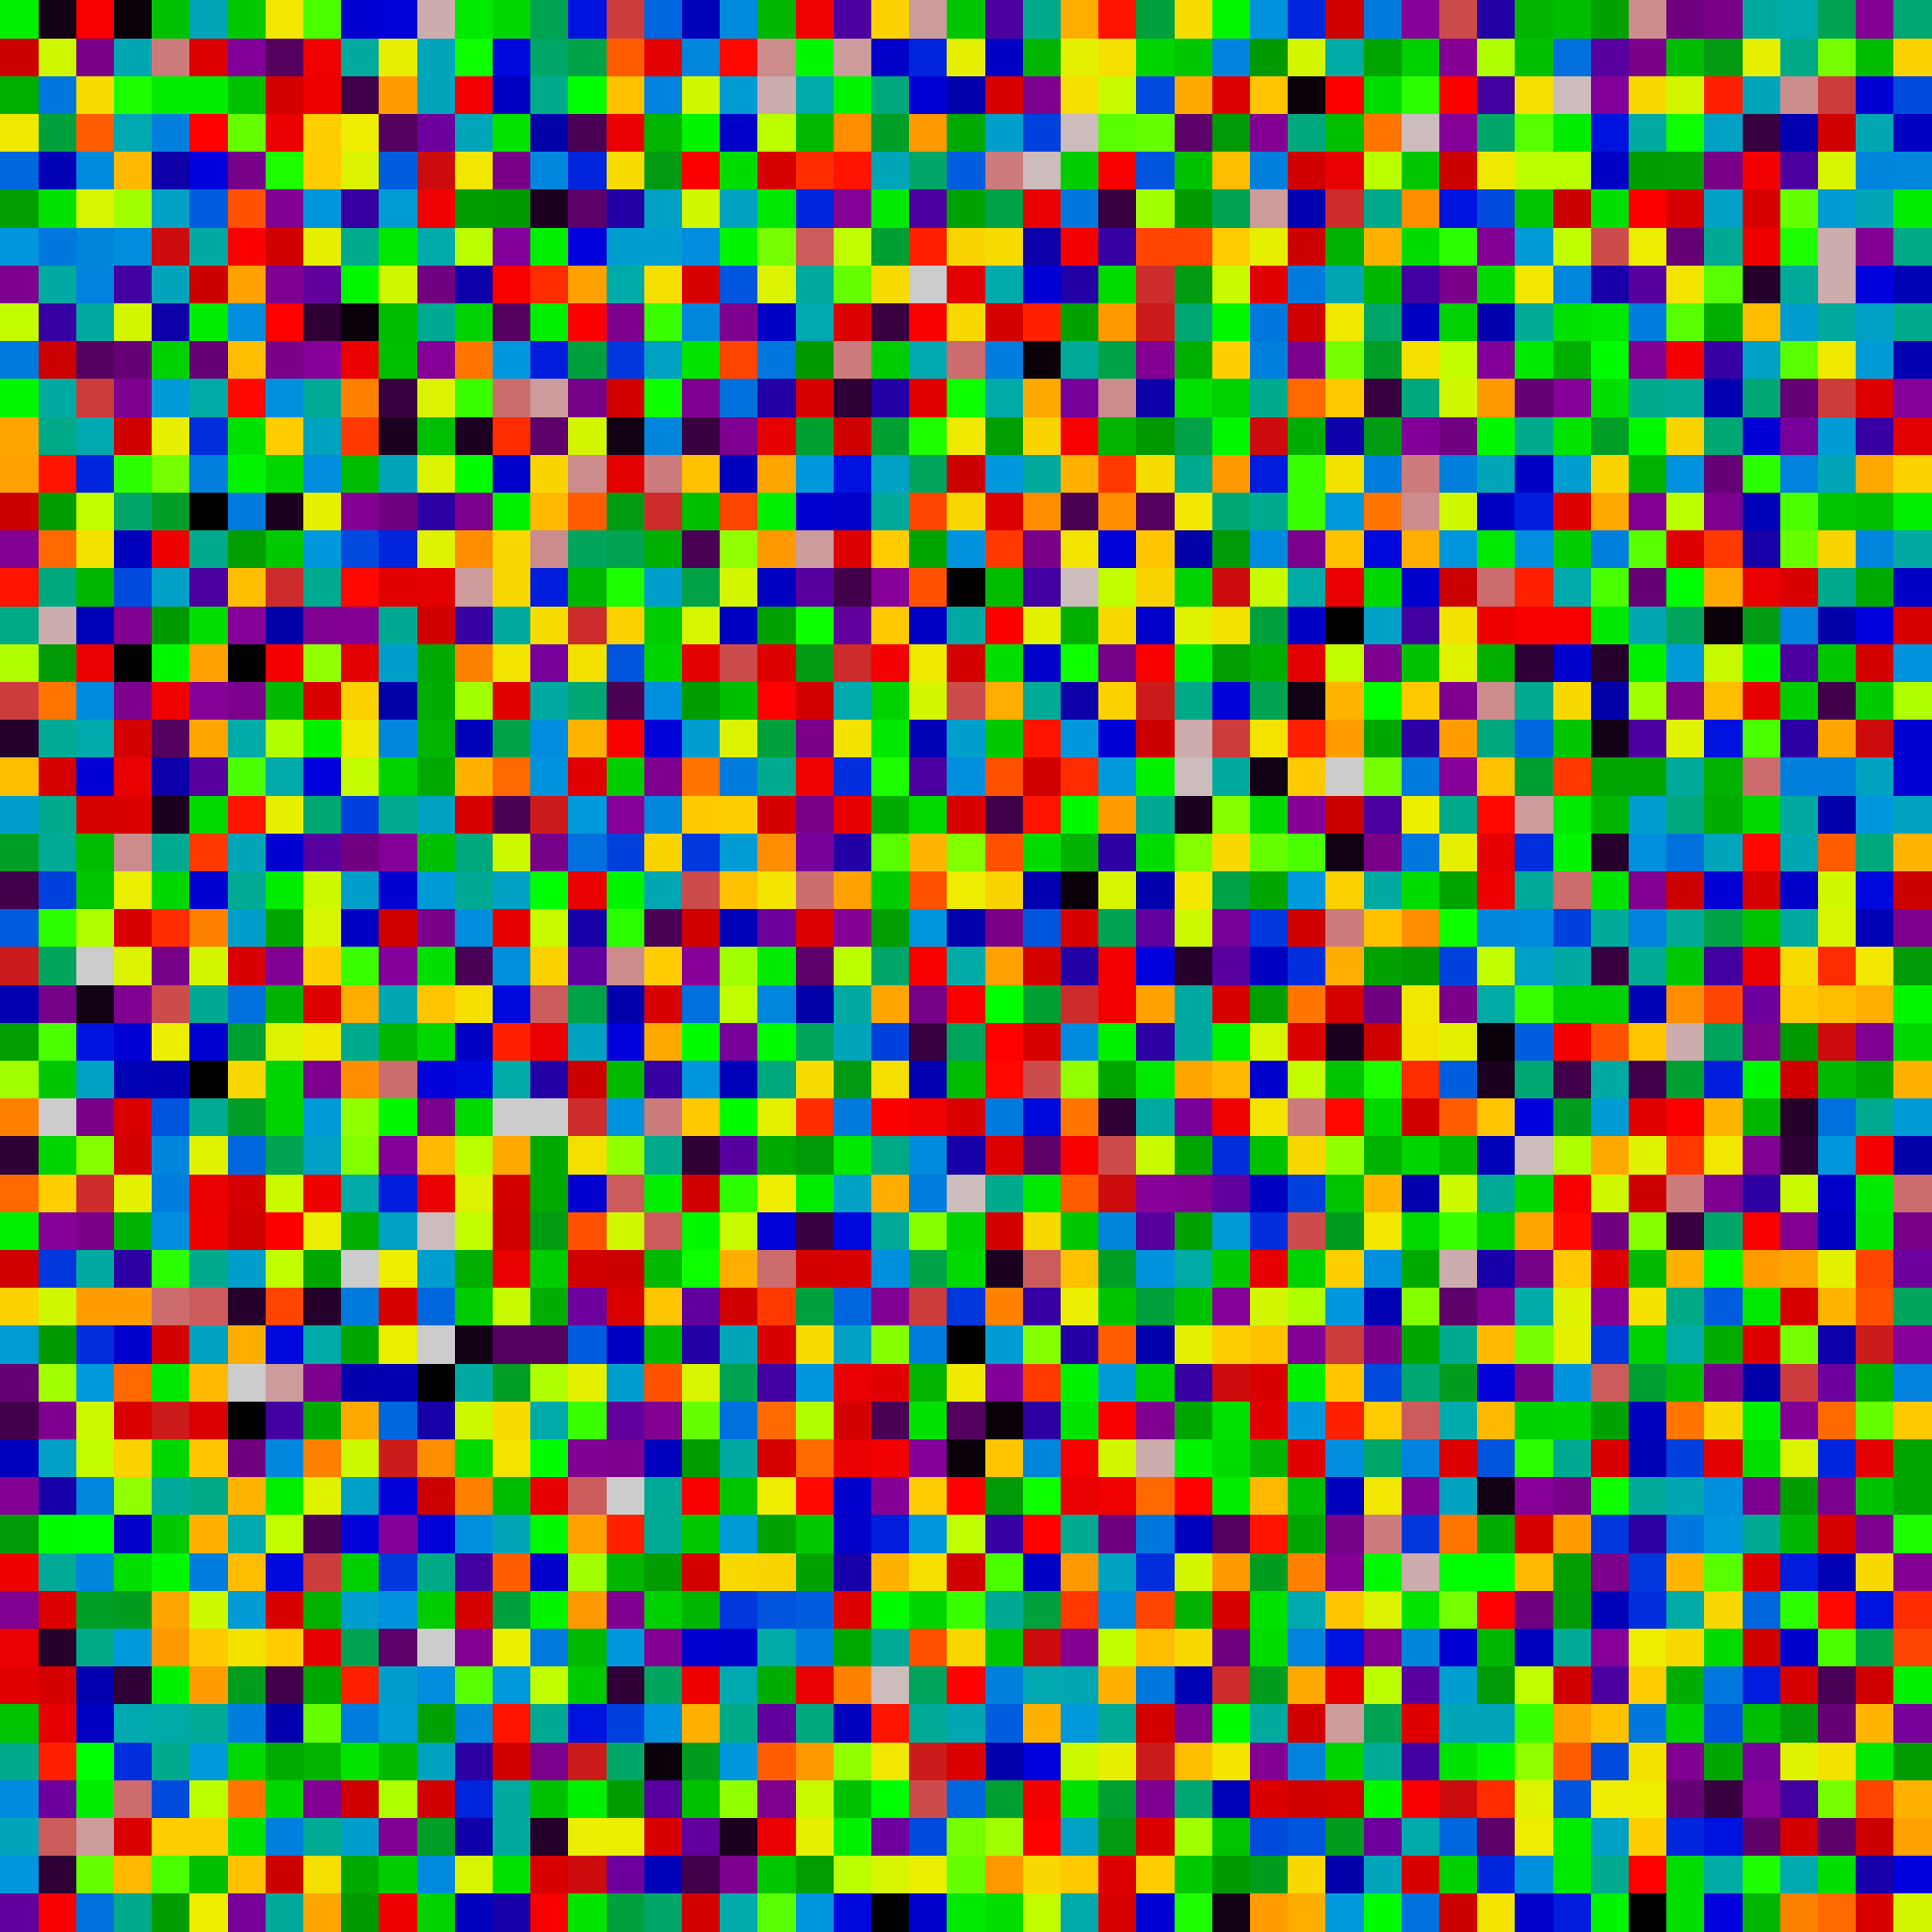
\includegraphics[width=0.9\linewidth]{figures/quantification/cmfd/cmfd-cells-reflector}
  \caption{}
  \label{fig:chap8-cmfd-cells}
\end{subfigure}
\caption[FSR discretization and CMFD cells for a 2$\times$2 colorset with a reflector]{\ac{FSR} discretization and \ac{CMFD} cells for a 2$\times$2 colorset with a water reflector.}
\label{fig:chap8-assm-fsrs-cmfd-cells}
\end{figure}


%%%%%%%%%%%%%%%%%%%%%%%%%%%%%%%%%%%%%%%%%%%%%%%%%%%%%%%%%%%%%%%%%%%%%%%%%%%%%%%
\section{Analysis of Multi-Group Results}
\label{sec:chap8-mg-results}


%%%%%%%%%%%%%%%%%%%%%%%%
\subsection{Eigenvalues}
\label{subsec:chap8-eigenvalues}

\begin{table}[h!]
  \centering
  \caption[OpenMOC eigenvalue bias for heterogeneous benchmarks]{OpenMOC eigenvalue bias $\Delta\rho$ for heterogeneous benchmarks with varying spatial homogenization schemes and energy group structures.}
  \small
  \label{table:chap8-openmoc-eigenvalues}
  \vspace{6pt}
  \begin{tabular}{l l S[table-format=6.0] S[table-format=6.0] S[table-format=6.0]}
  \toprule
  \rowcolor{lightgray}
  & & \multicolumn{3}{S[table-format=6.1]}{\cellcolor{lightgray} {$\bm{\Delta\rho}$ \textbf{[pcm]}}} \\
  \multirow{-2}{*}{\cellcolor{lightgray} \bf Benchmark} &
  \multirow{-2}{*}{\cellcolor{lightgray} \bf \ac{MGXS} Scheme} &
  {\cellcolor{lightgray} \bf 2-Group} &
  {\cellcolor{lightgray} \bf 8-Group} &
  {\cellcolor{lightgray} \bf 70-Group} \\
  \midrule
\multirow{3}{*}{\parbox{2.5cm}{1.6\% Assm}} & Infinite & 217 & 3 & -163 \\
& Null & 83 & -50 & -136 \\
& Degenerate & 88 & -50 & -136 \\
  \midrule
\multirow{3}{*}{\parbox{2.5cm}{3.1\% Assm}} & Infinite & 180 & -34 & -195 \\
& Null & 93 & -54 & -159 \\
& Degenerate & 99 & -54 & -159 \\
  \midrule
\multirow{3}{*}{\parbox{2.5cm}{3.1\% Assm w/ 20 BPs}} & Infinite & 1056 & 151 & -270 \\
& Null & -143 & -157 & -227 \\
& Degenerate & -190 & -159 & -223 \\
  \midrule
\multirow{3}{*}{\parbox{2.5cm}{2$\times$2 Colorset}} & Infinite & 355 & -149 & -298 \\
& Null & 10 & -146 & -266 \\
& Degenerate & -17 & -146 & -263 \\
  \midrule
  \multirow{3}{*}{\parbox{2.3cm}{2$\times$2 Colorset w/ Reflector}} & Infinite & 462 & 462 & \\
  & Null & & & \\
  & Degenerate & & & \\
  \midrule
  \multirow{3}{*}{\parbox{2cm}{\ac{BEAVRS} Full Core}} & Infinite & 497 & 497 & \\
  & Null & & & \\
  & Degenerate & & & \\
  \bottomrule
\end{tabular}
\end{table}


%%%%%%%%%%%%%%%%%%%%%%%%%%
\subsection{Fission Rates}
\label{subsec:chap8-fiss-rates}

\begin{table}[h!]
  \centering
  \caption[Maximum OpenMOC fission rate errors]{Maximum OpenMOC fission rate errors for varying spatial homogenization schemes and energy groups structures.}
  \small
  \label{table:chap8-openmoc-max-fiss-rates}
  \vspace{6pt}
  \begin{tabular}{l l c c c}
  \toprule
  \rowcolor{lightgray}
  & & \multicolumn{3}{c}{\cellcolor{lightgray} \textbf{Max Error [\%]}} \\
  \multirow{-2}{*}{\cellcolor{lightgray} \bf Benchmark} &
  \multirow{-2}{*}{\cellcolor{lightgray} \bf \ac{MGXS} Scheme} &
  {\cellcolor{lightgray} \bf 2-Group} &
  {\cellcolor{lightgray} \bf 8-Group} &
  {\cellcolor{lightgray} \bf 70-Group} \\
  \midrule
\multirow{3}{*}{\parbox{2.5cm}{1.6\% Assm}} & Infinite & 2.76E+00 & 7.56E-01 & 4.71E-01 \\
& Null & 2.76E+00 & 7.46E-01 & 4.71E-01 \\
& Degenerate & 1.87E+00 & 7.83E-01 & 3.90E-01 \\
  \midrule
\multirow{3}{*}{\parbox{2.5cm}{3.1\% Assm}} & Infinite & 3.10E+00 & 8.29E-01 & 5.41E-01 \\
& Null & 3.09E+00 & 8.17E-01 & 5.42E-01 \\
& Degenerate & 2.09E+00 & 8.68E-01 & 4.72E-01 \\
  \midrule
\multirow{3}{*}{\parbox{2.5cm}{3.1\% Assm w/ 20 BPs}} & Infinite & 2.10E+00 & 5.13E-01 & 4.42E-01 \\
& Null & 2.07E+00 & 5.43E-01 & 4.44E-01 \\
& Degenerate & 1.71E+00 & 6.47E-01 & 3.70E-01 \\
  \midrule
  \multirow{3}{*}{\parbox{2.5cm}{2$\times$2 Colorset}} & Infinite & 6.92E+00 & 2.23E+00 & 1.29E+00 \\
& Null & 7.04E+00 & 2.22E+00 & 1.30E+00 \\
& Degenerate & 4.39E+00 & 2.04E+00 & 1.25E+00 \\
  \midrule
  \multirow{3}{*}{\parbox{2.3cm}{2$\times$2 Colorset w/ Reflector}} & Infinite & 462 & 462 & \\
  & Null & & & \\
  & Degenerate & & & \\
  \midrule
  \multirow{3}{*}{\parbox{2cm}{\ac{BEAVRS} Full Core}} & Infinite & 497 & 497 & \\
  & Null & & & \\
  & Degenerate & & & \\
  \bottomrule
\end{tabular}
\end{table}

\begin{table}[h!]
  \centering
  \caption[Mean OpenMOC fission rate errors]{Mean OpenMOC fission rate errors for varying spatial homogenization schemes and energy groups structures.}
  \small
  \label{table:chap8-openmoc-mean-fiss-rates}
  \vspace{6pt}
  \begin{tabular}{l l c c c}
  \toprule
  \rowcolor{lightgray}
  & & \multicolumn{3}{c}{\cellcolor{lightgray} \textbf{Mean Error [\%]}} \\
  \multirow{-2}{*}{\cellcolor{lightgray} \bf Benchmark} &
  \multirow{-2}{*}{\cellcolor{lightgray} \bf \ac{MGXS} Scheme} &
  {\cellcolor{lightgray} \bf 2-Group} &
  {\cellcolor{lightgray} \bf 8-Group} &
  {\cellcolor{lightgray} \bf 70-Group} \\
  \midrule
\multirow{3}{*}{\parbox{2.5cm}{1.6\% Assm}} & Infinite & 5.09E-02 & 1.22E-02 & 7.47E-05 \\
& Null & 5.07E-02 & 1.20E-02 & 5.91E-05 \\
& Degenerate & 3.02E-02 & 1.09E-02 & 2.02E-03 \\
  \midrule
\multirow{3}{*}{\parbox{2.5cm}{3.1\% Assm}} & Infinite & 7.88E-02 & 1.89E-02 & 9.45E-04 \\
& Null & 7.81E-02 & 1.85E-02 & 8.94E-04 \\
& Degenerate & 4.50E-02 & 1.69E-02 & 3.36E-03 \\
  \midrule
\multirow{3}{*}{\parbox{2.5cm}{3.1\% Assm w/ 20 BPs}} & Infinite & 9.02E-02 & 1.55E-02 & 4.54E-03 \\
& Null & 8.83E-02 & 1.47E-02 & 4.45E-03 \\
& Degenerate & 1.71E-02 & 8.44E-03 & 4.15E-03 \\
  \midrule
  \multirow{3}{*}{\parbox{2.5cm}{2$\times$2 Colorset}} & Infinite & 4.02E-02 & -1.17E-02 & -4.78E-03 \\
& Null & 3.44E-02 & -1.30E-02 & -4.81E-03 \\
& Degenerate & -1.05E-01 & -2.78E-02 & -5.62E-03 \\
  \midrule
  \multirow{3}{*}{\parbox{2.3cm}{2$\times$2 Colorset w/ Reflector}} & Infinite & 462 & 462 & \\
  & Null & & & \\
  & Degenerate & & & \\
  \midrule
  \multirow{3}{*}{\parbox{2cm}{\ac{BEAVRS} Full Core}} & Infinite & 497 & 497 & \\
  & Null & & & \\
  & Degenerate & & & \\
  \bottomrule
\end{tabular}
\end{table}

\begin{figure}[h!]
\centering
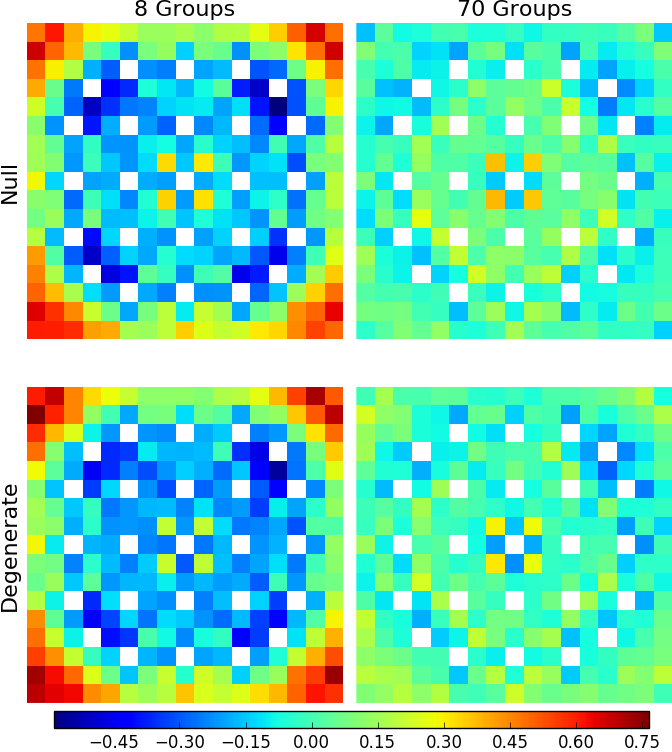
\includegraphics[width=\linewidth]{figures/quantification/assm-16/fiss-err}
\caption[Fission rate errors for a 1.6\% enriched assembly]{Fission rate errors for a 1.6\% enriched assembly.}
\label{fig:chap8-assm-1.6-fiss-err}
\end{figure}

\begin{figure}[h!]
\centering
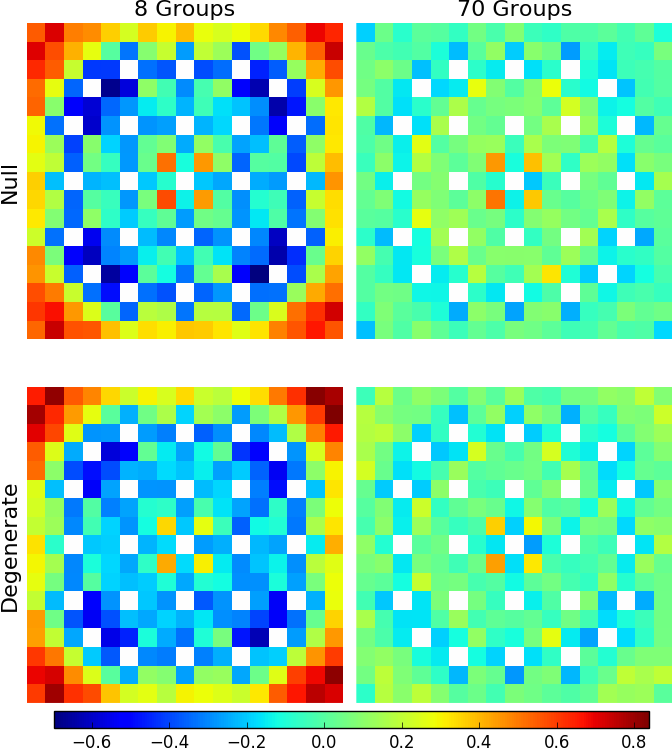
\includegraphics[width=\linewidth]{figures/quantification/assm-31/fiss-err}
\caption[Fission rate errors for a 3.1\% enriched assembly]{Fission rate errors for a 3.1\% enriched assembly.}
\label{fig:chap8-assm-3.1-fiss-err}
\end{figure}

\begin{figure}[h!]
\centering
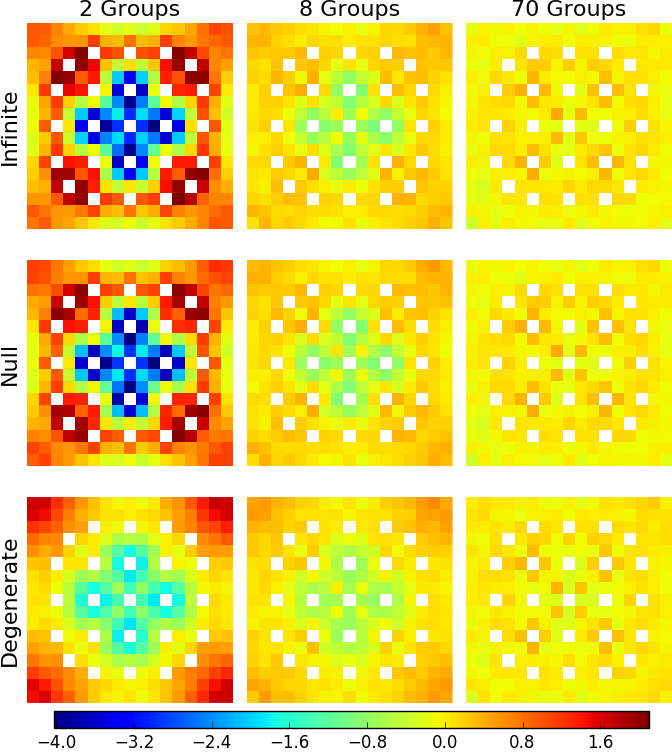
\includegraphics[width=\linewidth]{figures/quantification/assm-31-20BPs/fiss-err}
\caption[Fission rate errors for a 3.1\% enriched assembly with 20 BPs]{Fission rate errors for a 3.1\% enriched assembly with 20 BPs.}
\label{fig:chap8-assm-3.1-20BPs-fiss-err}
\end{figure}

\begin{figure}[h!]
\centering
\begin{subfigure}{.33\textwidth}
  \centering
  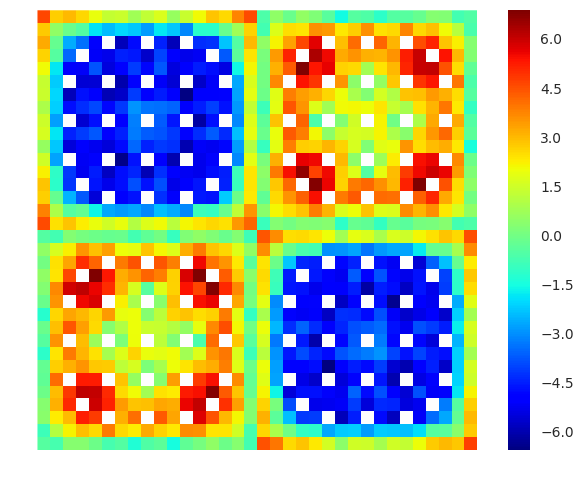
\includegraphics[width=\linewidth]{figures/quantification/2x2/infinite-fiss-err-2}
  \caption{}
  \label{fig:chap8-2x2-inf-fiss-2}
\end{subfigure}%
\begin{subfigure}{.33\textwidth}
  \centering
  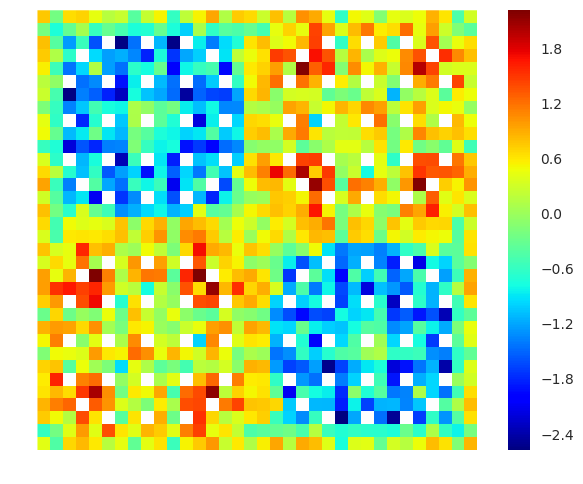
\includegraphics[width=\linewidth]{figures/quantification/2x2/infinite-fiss-err-8}
  \caption{}
  \label{fig:chap8-2x2-inf-fiss-8}
\end{subfigure}%
\begin{subfigure}{.33\textwidth}
  \centering
  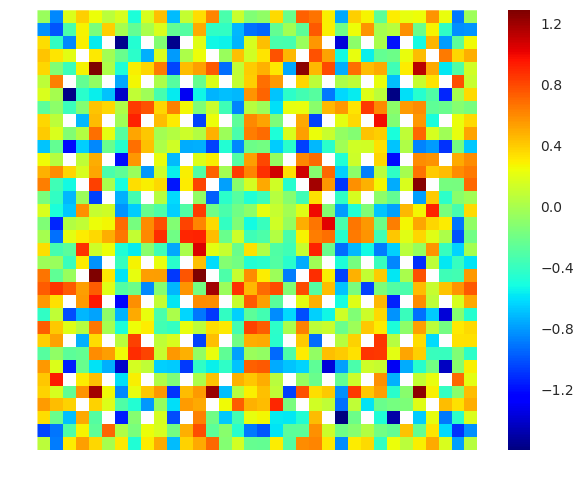
\includegraphics[width=\linewidth]{figures/quantification/2x2/infinite-fiss-err-70}
  \caption{}
  \label{fig:chap8-2x2-inf-fiss-70}
\end{subfigure}
\begin{subfigure}{.33\textwidth}
  \centering
  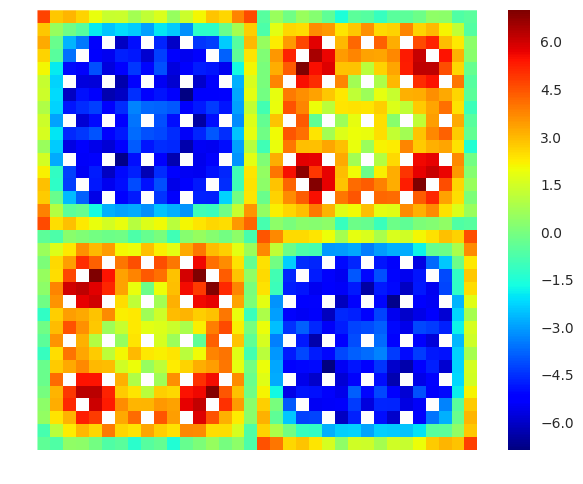
\includegraphics[width=\linewidth]{figures/quantification/2x2/null-fiss-err-2}
  \caption{}
  \label{fig:chap8-2x2-null-fiss-2}
\end{subfigure}%
\begin{subfigure}{.33\textwidth}
  \centering
  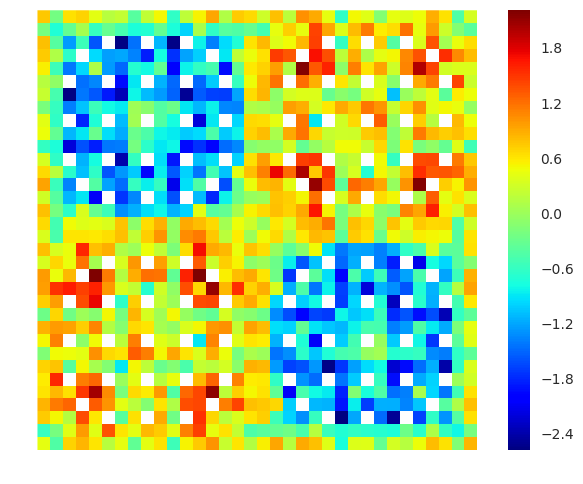
\includegraphics[width=\linewidth]{figures/quantification/2x2/null-fiss-err-8}
  \caption{}
  \label{fig:chap8-2x2-null-fiss-8}
\end{subfigure}%
\begin{subfigure}{.33\textwidth}
  \centering
  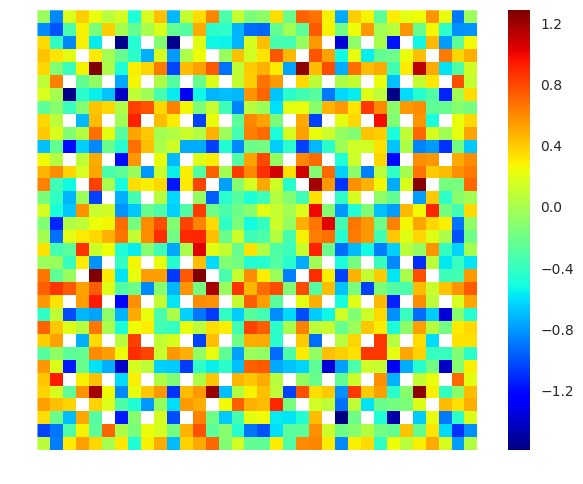
\includegraphics[width=\linewidth]{figures/quantification/2x2/null-fiss-err-70}
  \caption{}
  \label{fig:chap8-2x2-null-fiss-70}
\end{subfigure}
\begin{subfigure}{.33\textwidth}
  \centering
  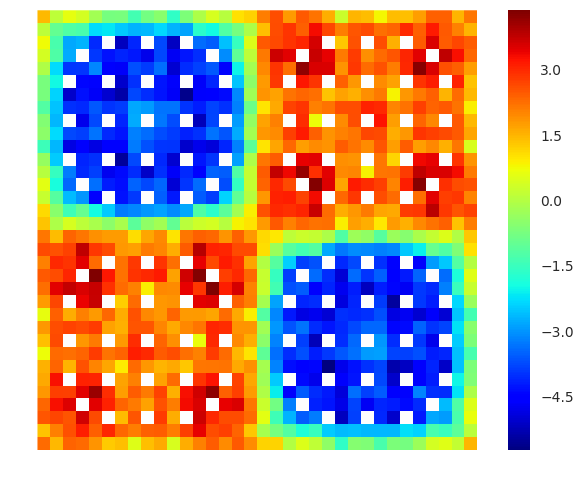
\includegraphics[width=\linewidth]{figures/quantification/2x2/degenerate-fiss-err-2}
  \caption{}
  \label{fig:chap8-2x2-degenerate-fiss-2}
\end{subfigure}%
\begin{subfigure}{.33\textwidth}
  \centering
  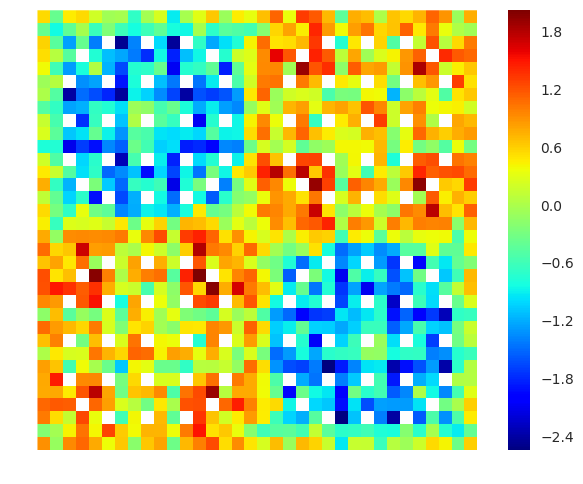
\includegraphics[width=\linewidth]{figures/quantification/2x2/degenerate-fiss-err-8}
  \caption{}
  \label{fig:chap8-2x2-degenerate-fiss-8}
\end{subfigure}%
\begin{subfigure}{.33\textwidth}
  \centering
  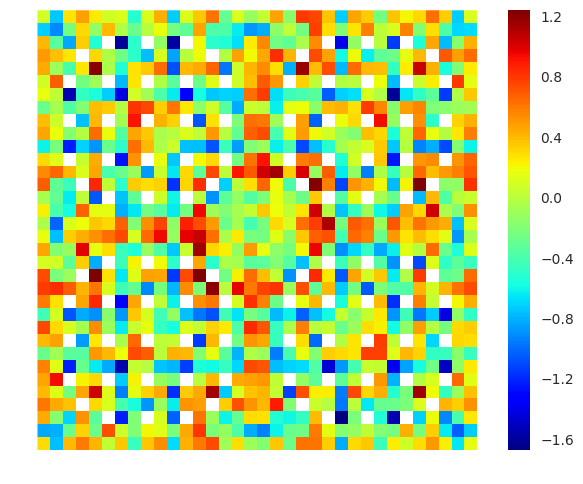
\includegraphics[width=\linewidth]{figures/quantification/2x2/degenerate-fiss-err-70}
  \caption{}
  \label{fig:chap8-2x2-degenerate-fiss-70}
\end{subfigure}
\caption[Fission rate errors for a 2$\times$2 colorset]{1.6\% enriched fuel pin (a), control rod guide tube (b), instrument tube (c) and burnable poison (d).}
\label{fig:chap8-2x2-fiss-err}
\end{figure}

\begin{itemize}[noitemsep]
  \item convergence rates for max/mean rel. err. for each benchmark
  \begin{itemize}[noitemsep]
    \item infinite vs. null vs. degenerate
    \item by energy group structure?
  \end{itemize}
  \item 2D heat maps of error distributions for each benchmark
  \begin{itemize}[noitemsep]
    \item infinite vs. null vs. degenerate
    \item by energy group structure?
  \end{itemize}
\end{itemize}

%%%%%%%%%%%%%%%%%%%%%%%%%%%%%%%%%%%%%%%%%%%%%
\subsection{U-238 Capture Rate Distributions}
\label{subsec:chap8-capt-rates}

\begin{table}[h!]
  \centering
  \caption[Maximum OpenMOC U-238 capture rate errors]{Maximum OpenMOC U-238 capture rate errors for varying spatial homogenization schemes and energy groups structures.}
  \small
  \label{table:chap8-openmoc-max-capt-rates}
  \vspace{6pt}
  \begin{tabular}{l l c c c}
  \toprule
  \rowcolor{lightgray}
  & & \multicolumn{3}{c}{\cellcolor{lightgray} \textbf{Max Error [\%]}} \\
  \multirow{-2}{*}{\cellcolor{lightgray} \bf Benchmark} &
  \multirow{-2}{*}{\cellcolor{lightgray} \bf \ac{MGXS} Scheme} &
  {\cellcolor{lightgray} \bf 2-Group} &
  {\cellcolor{lightgray} \bf 8-Group} &
  {\cellcolor{lightgray} \bf 70-Group} \\
  \midrule
\multirow{3}{*}{\parbox{2.5cm}{1.6\% Assm}} & Infinite & 2.60E+00 & 1.14E+00 & 8.54E-01 \\
& Null & 2.61E+00 & 1.14E+00 & 8.54E-01 \\
& Degenerate & 9.07E-01 & 3.88E-01 & 2.99E-01 \\
  \midrule
\multirow{3}{*}{\parbox{2.5cm}{3.1\% Assm}} & Infinite & 2.56E+00 & 1.24E+00 & 9.52E-01 \\
& Null & 2.56E+00 & 1.24E+00 & 9.52E-01 \\
& Degenerate & 8.14E-01 & 4.75E-01 & 3.39E-01 \\
  \midrule
\multirow{3}{*}{\parbox{2.5cm}{3.1\% Assm w/ 20 BPs}} & Infinite & 3.00E+00 & 1.11E+00 & 7.40E-01 \\
& Null & 3.02E+00 & 1.11E+00 & 7.40E-01 \\
& Degenerate & 1.36E+00 & 6.19E-01 & 2.96E-01 \\
  \midrule
  \multirow{3}{*}{\parbox{2.5cm}{2$\times$2 Colorset}} & Infinite & 4.12E+00 & 2.16E+00 & 1.75E+00 \\
& Null & 4.20E+00 & 2.17E+00 & 1.75E+00 \\
& Degenerate & 2.61E+00 & 1.29E+00 & 1.30E+00 \\
  \midrule
  \multirow{3}{*}{\parbox{2.3cm}{2$\times$2 Colorset w/ Reflector}} & Infinite & 462 & 462 & \\
  & Null & & & \\
  & Degenerate & & & \\
  \midrule
  \multirow{3}{*}{\parbox{2cm}{\ac{BEAVRS} Full Core}} & Infinite & 497 & 497 & \\
  & Null & & & \\
  & Degenerate & & & \\
  \bottomrule
\end{tabular}
\end{table}

\begin{table}[h!]
  \centering
  \caption[Mean OpenMOC U-238 capture rate errors]{Mean OpenMOC U-238 capture rate errors for varying spatial homogenization schemes and energy groups structures.}
  \small
  \label{table:chap8-openmoc-mean-capt-rates}
  \vspace{6pt}
  \begin{tabular}{l l c c c}
  \toprule
  \rowcolor{lightgray}
  & & \multicolumn{3}{c}{\cellcolor{lightgray} \textbf{Mean Error [\%]}} \\
  \multirow{-2}{*}{\cellcolor{lightgray} \bf Benchmark} &
  \multirow{-2}{*}{\cellcolor{lightgray} \bf \ac{MGXS} Scheme} &
  {\cellcolor{lightgray} \bf 2-Group} &
  {\cellcolor{lightgray} \bf 8-Group} &
  {\cellcolor{lightgray} \bf 70-Group} \\
  \midrule
\multirow{3}{*}{\parbox{2.5cm}{1.6\% Assm}} & Infinite & 3.41E-02 & 1.65E-02 & 1.17E-02 \\
& Null & 3.41E-02 & 1.65E-02 & 1.17E-02 \\
& Degenerate & 8.19E-03 & 5.01E-04 & 4.37E-04 \\
  \midrule
\multirow{3}{*}{\parbox{2.5cm}{3.1\% Assm}} & Infinite & 3.95E-02 & 1.98E-02 & 1.46E-02 \\
& Null & 3.94E-02 & 1.98E-02 & 1.46E-02 \\
& Degenerate & 8.15E-03 & -2.87E-04 & 4.77E-04 \\
  \midrule
\multirow{3}{*}{\parbox{2.5cm}{3.1\% Assm w/ 20 BPs}} & Infinite & -8.62E-03 & -3.80E-03 & -2.13E-03 \\
& Null & -7.91E-03 & -3.75E-03 & -2.17E-03 \\
& Degenerate & -3.50E-03 & -3.00E-03 & 2.29E-04 \\
  \midrule
  \multirow{3}{*}{\parbox{2.5cm}{2$\times$2 Colorset}} & Infinite & 1.20E-01 & 1.73E-03 & 1.16E-02 \\
& Null & 1.28E-01 & 1.87E-03 & 1.16E-02 \\
& Degenerate & 9.84E-02 & -8.66E-03 & 6.95E-03 \\
  \midrule
  \multirow{3}{*}{\parbox{2.3cm}{2$\times$2 Colorset w/ Reflector}} & Infinite & 462 & 462 & \\
  & Null & & & \\
  & Degenerate & & & \\
  \midrule
  \multirow{3}{*}{\parbox{2cm}{\ac{BEAVRS} Full Core}} & Infinite & 497 & 497 & \\
  & Null & & & \\
  & Degenerate & & & \\
  \bottomrule
\end{tabular}
\end{table}


\begin{figure}[h!]
\centering
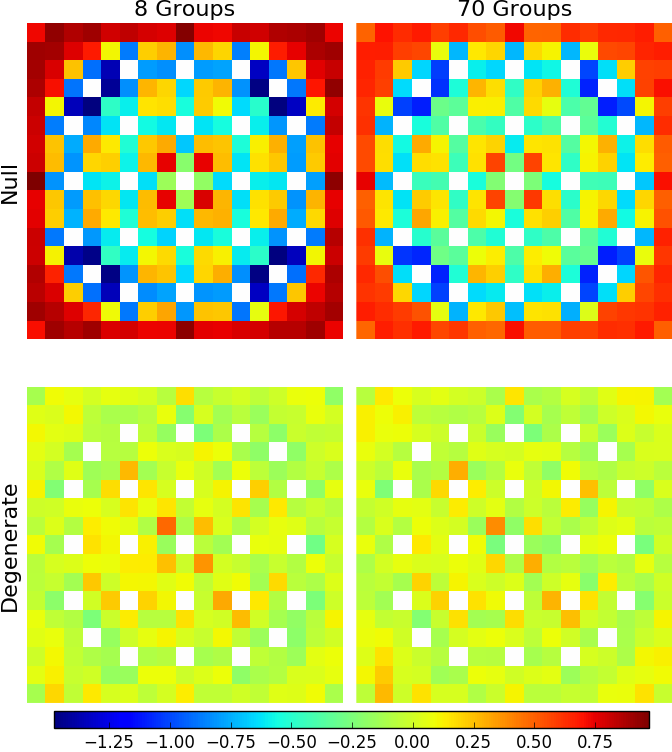
\includegraphics[width=\linewidth]{figures/quantification/assm-16/capt-err}
\caption[U-238 capture rate errors for a 1.6\% enriched assembly]{U-238 capture rate errors for a 1.6\% enriched assembly.}
\label{fig:chap8-assm-1.6-capt-err}
\end{figure}

\begin{figure}[h!]
\centering
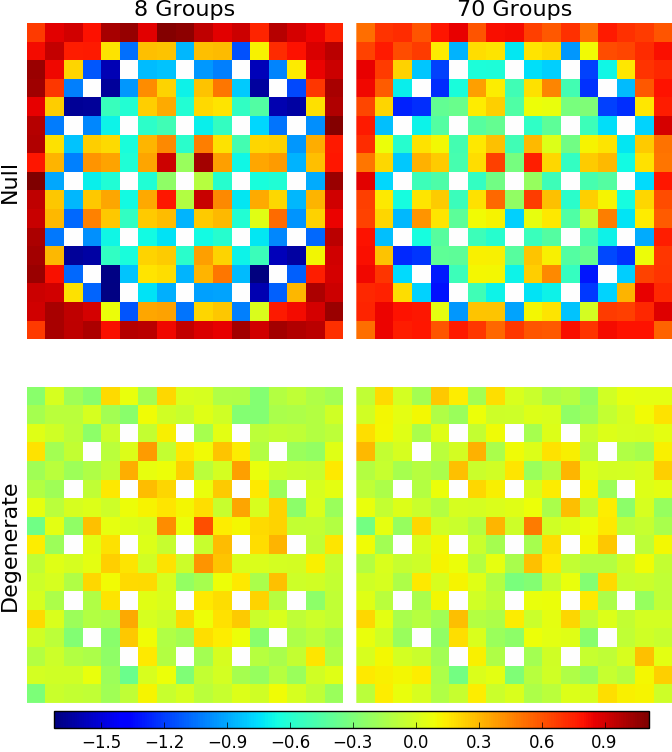
\includegraphics[width=\linewidth]{figures/quantification/assm-31/capt-err}
\caption[U-238 capture rate errors for a 3.1\% enriched assembly]{U-238 capture rate errors for a 3.1\% enriched assembly.}
\label{fig:chap8-assm-3.1-capt-err}
\end{figure}

\begin{figure}[h!]
\centering
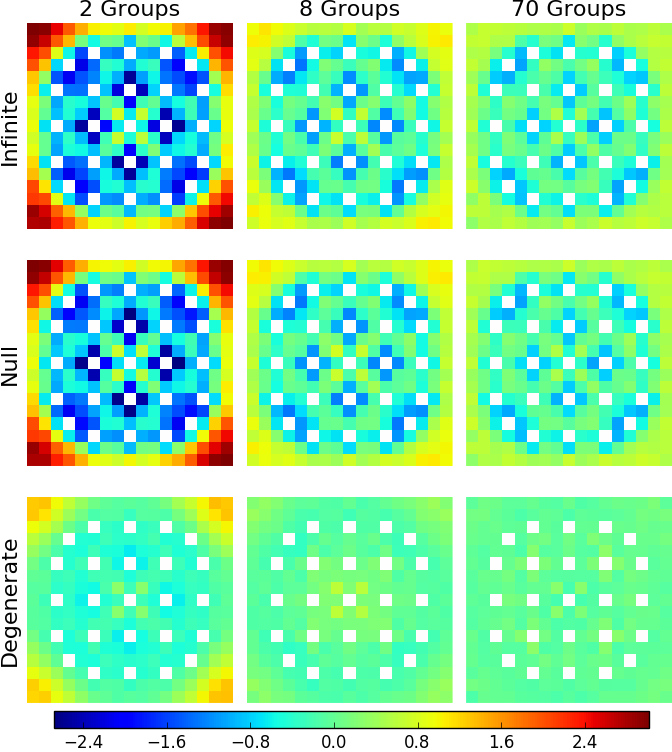
\includegraphics[width=\linewidth]{figures/quantification/assm-31-20BPs/capt-err}
\caption[U-238 capture rate errors for a 3.1\% enriched assembly with 20 BPs]{U-238 capture rate errors for a 3.1\% enriched assembly with 20 BPs.}
\label{fig:chap8-assm-3.1-20BPs-capt-err}
\end{figure}


\begin{figure}[h!]
\centering
\begin{subfigure}{.33\textwidth}
  \centering
  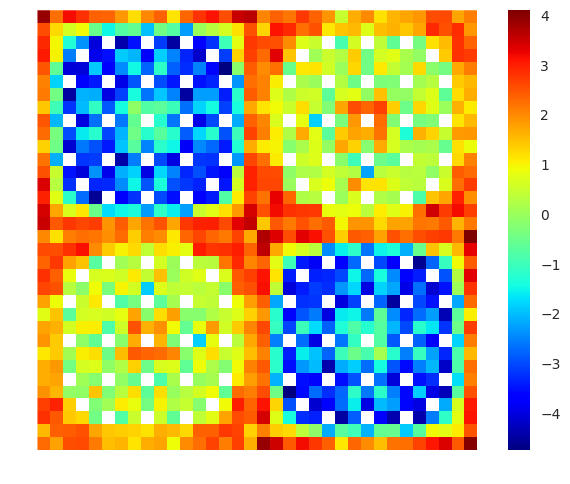
\includegraphics[width=\linewidth]{figures/quantification/2x2/infinite-capt-err-2}
  \caption{}
  \label{fig:chap8-2x2-inf-capt-2}
\end{subfigure}%
\begin{subfigure}{.33\textwidth}
  \centering
  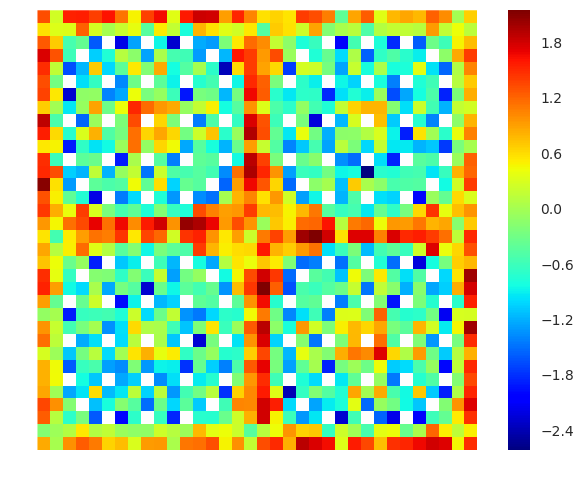
\includegraphics[width=\linewidth]{figures/quantification/2x2/infinite-capt-err-8}
  \caption{}
  \label{fig:chap8-2x2-inf-capt-8}
\end{subfigure}%
\begin{subfigure}{.33\textwidth}
  \centering
  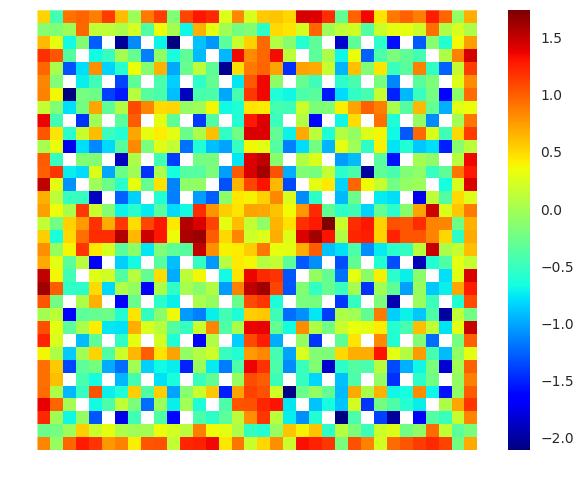
\includegraphics[width=\linewidth]{figures/quantification/2x2/infinite-capt-err-70}
  \caption{}
  \label{fig:chap8-2x2-inf-capt-70}
\end{subfigure}
\begin{subfigure}{.33\textwidth}
  \centering
  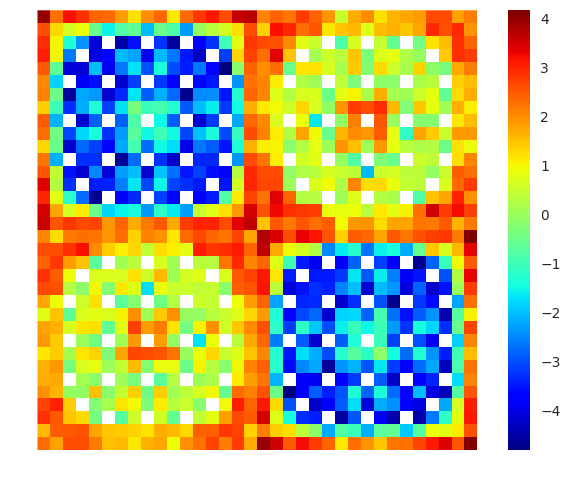
\includegraphics[width=\linewidth]{figures/quantification/2x2/null-capt-err-2}
  \caption{}
  \label{fig:chap8-2x2-null-capt-2}
\end{subfigure}%
\begin{subfigure}{.33\textwidth}
  \centering
  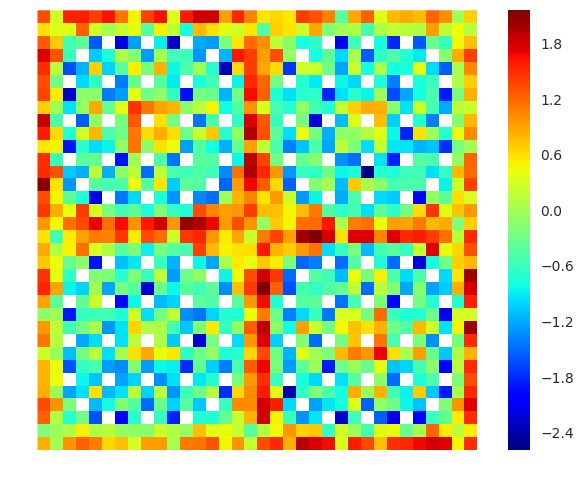
\includegraphics[width=\linewidth]{figures/quantification/2x2/null-capt-err-8}
  \caption{}
  \label{fig:chap8-2x2-null-capt-8}
\end{subfigure}%
\begin{subfigure}{.33\textwidth}
  \centering
  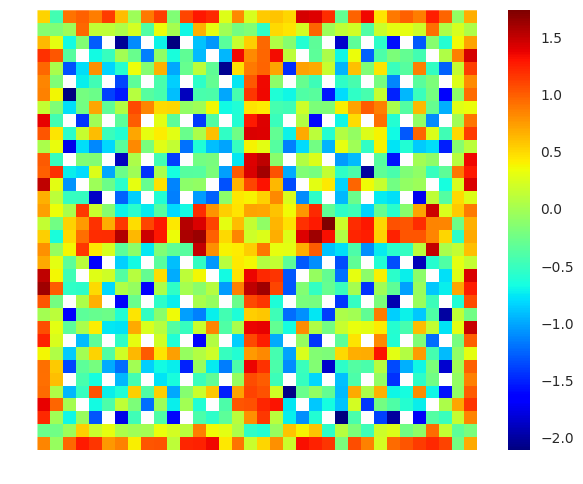
\includegraphics[width=\linewidth]{figures/quantification/2x2/null-capt-err-70}
  \caption{}
  \label{fig:chap8-2x2-null-capt-70}
\end{subfigure}
\begin{subfigure}{.33\textwidth}
  \centering
  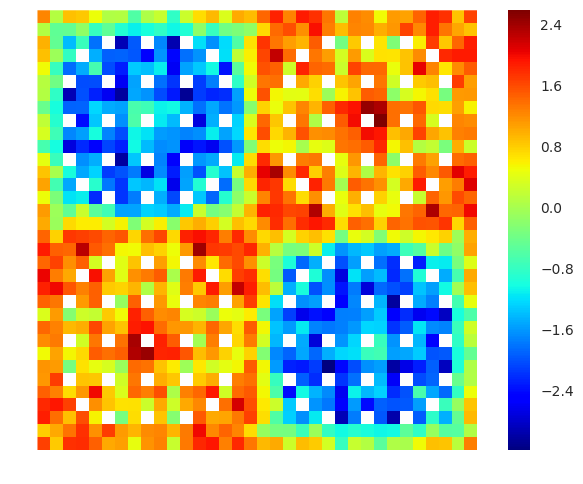
\includegraphics[width=\linewidth]{figures/quantification/2x2/degenerate-capt-err-2}
  \caption{}
  \label{fig:chap8-2x2-degenerate-capt-2}
\end{subfigure}%
\begin{subfigure}{.33\textwidth}
  \centering
  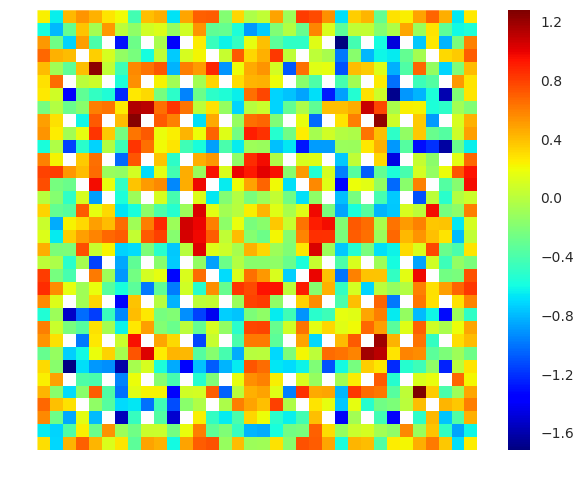
\includegraphics[width=\linewidth]{figures/quantification/2x2/degenerate-capt-err-8}
  \caption{}
  \label{fig:chap8-2x2-degenerate-capt-8}
\end{subfigure}%
\begin{subfigure}{.33\textwidth}
  \centering
  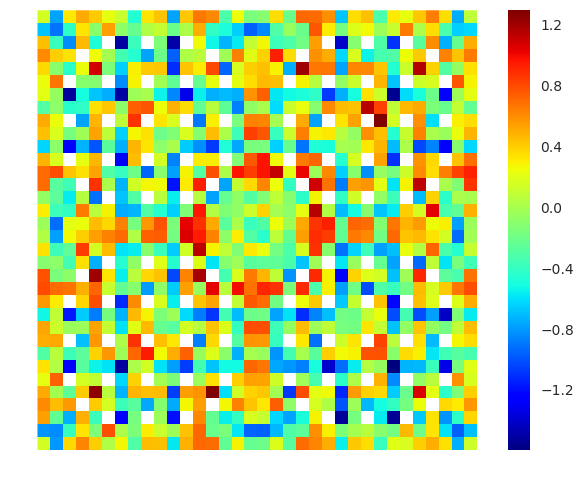
\includegraphics[width=\linewidth]{figures/quantification/2x2/degenerate-capt-err-70}
  \caption{}
  \label{fig:chap8-2x2-degenerate-capt-70}
\end{subfigure}
\caption[U-238 capture rate errors for a 2$\times$2 colorset]{1.6\% enriched fuel pin (a), control rod guide tube (b), instrument tube (c) and burnable poison (d).}
\label{fig:chap8-2x2-capt-err}
\end{figure}


\begin{itemize}[noitemsep]
  \item convergence rates for max/mean rel. err. for each benchmark
  \begin{itemize}[noitemsep]
    \item infinite vs. null vs. degenerate
    \item by energy group structure?
  \end{itemize}
  \item 2D heat maps of error distributions for each benchmark
  \begin{itemize}[noitemsep]
    \item infinite vs. null vs. degenerate
    \item by energy group structure?
  \end{itemize}
\end{itemize}

%-infinite vs. null vs. degenerate
%-conv rates for MGXS in each case - choose worst groups
%  -compare back to pin power error conv. rates
%  -convergence rates for infinite vs. null vs. degenerate